\documentclass[letter,12pt]{article}
\usepackage[letterpaper,right=1.25in,left=1.25in,top=1in,bottom=1in]{geometry}
\usepackage{setspace}

\usepackage[utf8]{inputenc}   % allows input of special characters from keyboard (input encoding)
\usepackage[T1]{fontenc}      % what fonts to use when printing characters       (output encoding)
\usepackage{amsmath}          % facilitates writing math formulas and improves the typographical quality of their output
\usepackage{url}              % adds line breaks to long urls
\usepackage[pdftex]{graphicx} % enhanced support for graphics
\usepackage{tikz}             % Easier syntax to draw pgf files (invokes pgf automatically)
\usetikzlibrary{arrows}

\usepackage{mathptmx}           % set font type to Times
\usepackage[scaled=.90]{helvet} % set font type to Times (Helvetica for some special characters)
\usepackage{courier}            % set font type to Times (Courier for other special characters)

\usepackage[longnamesfirst, sort]{natbib}\bibpunct[]{(}{)}{,}{a}{}{;} % handles biblio and references 

\usepackage{rotating}         % sideway tables and figures that take a full page
\usepackage{caption}          % allows multipage figures and tables with same caption (\ContinuedFloat)

\usepackage{dcolumn}          % needed for apsrtable and stargazer tables from R to compile
\usepackage{arydshln}         % dashed lines in tables (hdashline, cdashline{3-4}, 
                              %see http://tex.stackexchange.com/questions/20140/can-a-table-include-a-horizontal-dashed-line)
                              % must be loaded AFTER dcolumn, 
                              %see http://tex.stackexchange.com/questions/12672/which-tabular-packages-do-which-tasks-and-which-packages-conflict


\newcommand{\mc}{\multicolumn}

%% TO ADD NOTES IN TEXT
\usepackage[colorinlistoftodos, textsize=small]{todonotes}
\newcommand{\emm}[1]{\todo[color=blue!30, inline]{\textbf{To do:} #1}}

% agradecimientos
% Sebasti\'an Soto Velasco, ex-director jur\'idico de del ministerio secretaría general de la presidencia
% Roberto Bustos, Secretario de la Comisi\'on de Hacienda del Senado
% Alvaro Villarroel, staff Comisi\'on de Hacienda del Senado
% Tercer staff de Comisi\'on de Hacienda del Senado
% Dip. Patricio Vallesp\'in
% Dip. 1er vice-presidente de la C\'amara de Diputados


\begin{document}

\title{Presidential obstruction of the \\agenda in Chile's Congress\thanks{Prepared for presentation at the Instituto de Ciencia Pol\'itica, Universidad Cat\'olica, Santiago de Chile. The authors are grateful to Ernesto Calvo, Jos\'e Antonio Cheibub, and participants at the Comparative Politics Workshop of the University of Illinois at Urbana-Champaign for useful comments and critiques. Eric Magar acknowledges financial support from the Asociaci\'on Mexicana de Cultura A.C.\ and CONACYT's Sistema Nacional de Investigadores. The authors bear sole responsibility for mistakes and shortcomings in the study.}}
\author{Eric Magar \\ ITAM \and
        Valeria Palanza \\ Univ.\ Cat\'olica de Chile \and  
        Gisela Sin \\ Univ.\ of Illinois, Urbana-Champaign 
}
\date{\today}
\maketitle

% \begin{center} \textbf{$\rightarrow$~~Preliminary draft~~$\leftarrow$} \\ (please inquire for new version, \small{\url{emagar@itam.mx}})  \end{center}

\begin{abstract}
\noindent Unlike presidents with mostly (or only) reactive formal powers in the legislative arena, Chile's enjoys formidable proactive ones. Among them is the urgency authority. A bill declared urgent confronts legislators with a short deadline to discuss and vote it. Urgency, research has shown, correlates with the odds of bill passage, and most executive-initiated legislation becomes urgent at some stage. Comparing the Chilean urgency authority to others in the region reveals the absence of a penalty for non-compliance. Urgency messages in Chile appear as cheap talk unless presidents can persuade legislators that costs indeed exist. Inspecting original data on the decision to declare legislation urgent sheds light on the disconnect between frequent usage and institutional void. I do not answer what makes the urgency consequential satisfactorily, but the attempt reveals suggestive patterns and raises puzzles worth investigating further. 
\end{abstract}

% para ges y valeria: opción 1 es usar shareLatex; opción 2 es buscar sugerencias para colaborar en web via word; opción 3 es editar en word dándoles unas instrucciones básicas de qué no tocar; opción 4 es sacar los párrafos de texto con menciones de tables y figures (que deben ver en el pdf)... voy por ésta ahora

 %Inspection of original data on urgency incidence to investigate the decision to declare or not legislation urgent, an aspect that has received less scholarly attention. Analysis of original data distinguishes messages in the 1998--2014 period that set forth urgency (40\% of 20 thousand), messages that changed the deadline (29\%), and messages to withdraw the bill's urgency (31\%). Isolating bill and session traits that correlate with urgencies sheds light on the president's power to constantly obstruct the legislative agenda and its use in executive-legislative negotiation with separation of power. 

% comentarios de Calvo
%Comentarios a Magar: Presidential obstruction of the agenda in Chile’s Congress
%Buenísimo el paper. Siempre me pareció muy interesante el tema de las urgencias y no existen análisis sistemáticos de estos procesos. Tengo muchas ganas de ver el libro completo una vez que esté terminado. 
%En términos generales me gusta mucho la perspectiva y el modelo es interesante. El juego está descripto con poco detalle (supongo que eso viene en otros capítulos) así que la presentación de la Figura 2 y su discusión en las páginas 10 y 11 siguen siendo un poco crípticos. La intuición se entiende, pero el hecho de que en distintos sistemas k y o toman distintos valores y producen distintos equilibrios necesita más fundamentación (de nuevo, asumo que eso viene de capítulos anteriores del libro). 
%El capítulo preguntando porque los legisladores toman en consideración las “urgencias” cuando a diferencia de Brasil o Uruguay no existe un mecanismo de sanción si ellos “shirk”. No tenemos respuesta a lo largo del capítulo y mi impresión es que se necesita un poco mas de data cualitativa (algunas entrevistas o discusiones de diarios de sesiones) que digan porque los legisladores atienden al pedido del presidente. Esto quizá afecte como pensas el modelo de la Figura 2 y te convendría resolverlo antes de cerrar el capítulo.
%Mi preocupación principal está en la forma en que usas la data y como estimas el modelo. Las “urgencias” son un mecanismo para presionar al Congreso para que actúe y, por tanto, tienen que ser modelados con una función de tiempo. Lo más natural para mí sería utilizar un “mixture” model que mide al mismo tiempo la “tasa” de aprobación y el “tiempo” de aprobación (te anexo un artículo en el cual hacemos esto para el caso de Uruguay con Chasquetti). Entiendo que las “urgencias” son una forma de presionar al Congreso para resolver favorablemente, pero la discusión sobre el “scheduling” del plenario también refiere al problema del costo de oportunidad de tratar los proyectos del Presidente en lugar de los proyectos de los legisladores. Sin embargo, todos los Congresos tienen mecanismos para permitir que los “pet projects” sean aprobados cuando hay tiempos limitados en el plenario. En Brasil las comisiones pueden dar aprobación final a una gran cantidad de projectos (“terminativa”) para evitar consumir el tiempo del plenario. En Argentina el artículo 133 del reglamento permite votar en paquete proyectos que tienen dictamen de comisión y no tienen objeciones ni enmiendas. Por lo tanto, existen cambios en las reglas que les permiten a los legisladores “circunvent” las restricciones de tiempo del plenario. Para mi es necesario modelar el éxito relativo y el tiempo de aprobación para ver que es lo que están haciendo las urgencias.
%Esto también quiere decir que el modelo de estimación debería ser al nivel de proyecto de ley y no un OLS con sumas de instancias. Sino me equivoco tenes toda esa data, el N es mas grande y además te permite combinar data a nivel de proyecto, de legislador y de Congreso. Así que a mi juicio conviene cambiar la estrategia de estimación. 
%Por lo demás, me parece un excelente artículo y me muero de ganas de ver el libro.
%Abrazo. E.  

% Joy comments
% Need to explain tables better
% Need to explain figures better
% Get interviews to offer intuitions on what numbers can't explain
% EMM: should simplify argument---absent a cost given r=x_0 and schadule unchanged, k>o necessary.

\onehalfspacing

\noindent Threats are promises to inflict harm unless the receiver transfers welfare to whoever stated the threat. From an economic perspective, action in accordance with the threatener's wishes should follow so long as the harm exceeds the welfare transfer demanded---else the threatened person is better off enduring the penalty \citep{dahl.ConceptPower1957,friedrich.1941,schelling.1960}. Empty threats are those failing to fulfil the large penalty condition. Finding frequent compliance to empty threats would puzzle proponents of this strategic stylization of power relations. This paper detects one such puzzle in urgency authority incidence in Chile. 

This paper compares the urgency authority in Chile to those found in a few other constitutions of the Americas. A president with urgency authority can remove obstacles preventing floor consideration of legislative proposals. One striking finding of this institutional contrast is how Chilean urgency urgency messages carry no formal penalty whatsoever for non-compliance, and therefore have the status of empty threats to Congress, otherwise known as cheap talk. 

Yet inspection of recent urgency message incidence reveals a strikingly high frequency: one of every five bills in Congress received some form of executive urgency at some stage (and often at several stages) of the legislative process; and more than two-thirds of executive proposals did. Adding a layer to the puzzle, Congress in fact complied with a significant number of urgency messages. Why would presidents resort so remarkably frequently to the institutionally inconsequential urgency authority? And why would legislators comply so often with empty executive threats?

The paper proceeds thus. Section 1 briefly reviews empirical studies of the urgency authority, spotting a major obstacle to measure its effects. Section 2 offers a theoretical framework to compare the urgency authority across constitutions. Highlighting two key institutional features---the reversionary policy and reversionary schedule applicable when the assembly misses the urgent deadline---reveals a flaw in the Chilean (and possibly Mexican) variants, compared to the Brazilian, Colombian, and Uruguayan: urgency messages are cheap talk. The framework also shows that the existence of indirect costs---what \citet{neustadt.1990} calls \emph{presidential persuation}---is one way to restore the Chilean institution's bite. Section 3 looks at urgency degrees, another feature of Chile's institution, and speculates about their potential to render the urgency authority consequential. Section 4 introduces an original dataset of bill histories and urgency messages in Chile in the 1998--2014 period. Many puzzles arise from the descriptive statistics on bill initiation, bill passage, and urgency usage. One is the disconnect between a possibly inconsequential institution and the remarkable frequency of its use. Section 5 inspects committee reporting following different types of urgency messages. Analysis shows that, far from inconsequential, the urgency authority indeed lets Chilean presidents determine legislative scheduling. Section 6 offers closing remarks. 

\section{Reading and amending proposals}

We stylize the evolution of a legislative proposal, from introduction to passage. We illustrate with the simple example of a proposal that gives rise to two amendments, one upon referral to the standing committee, another later in the process. The proposal consists of three articles, as follows. 

\begin{center}
\noindent \begin{tabular}{llc}
       & original version                   & amendments                                       \\ \hline
Art 1. & appropriate \$200                  & \$300                                            \\
Art 2. & split in two equal parts           & $(\frac{1}{4}, \frac{3}{4})$ split \\
Art 3. & one for students, one for teachers & ---                                              \\
\end{tabular}
\end{center}

\noindent If approved, students and teachers receive a \$100 grant each. Adding tension, assume that the C\'amara majority has committed \$150 to teachers. An amendment (\emph{indicación} in Chilean legislative  parlance) to art.\ 1 is therefore presented, increasing the appropriation to meet the commitment. One problem arises: only the executive is entitled to introduce legislation (and amendments to legislation) increasing spending. The committee chair decides on the admissibility of amendments on such grounds---a decision that the C\'amara's presiding officer can override.\footnote{Congress' organic law (arts.\ 24 and 25) might leave discretion to committee chairs and presiding officer to declare amendments inadmissible. Non-germane amendments, or that increase spending, or those falling in areas of exclusive executive initiative, are explicitly mentioned as inadmissible.} 

This is a form of ex-ante veto: if unwilling to appropriate extra money, the presideingt officer can simply declare the amendment inadmissibile. In which case, the distributive route remains practicable: less for students, more for teachers. An amendment to art.\ 2, such that teachers get three-fourths of the \$200 appropriation, honors the commitment---at the students' expense. By leaving spending untouched, it might be harder for the presiding officer to argue in favor of not admitting the second amendment. 


\begin{sidewaysfigure}
  \centering
    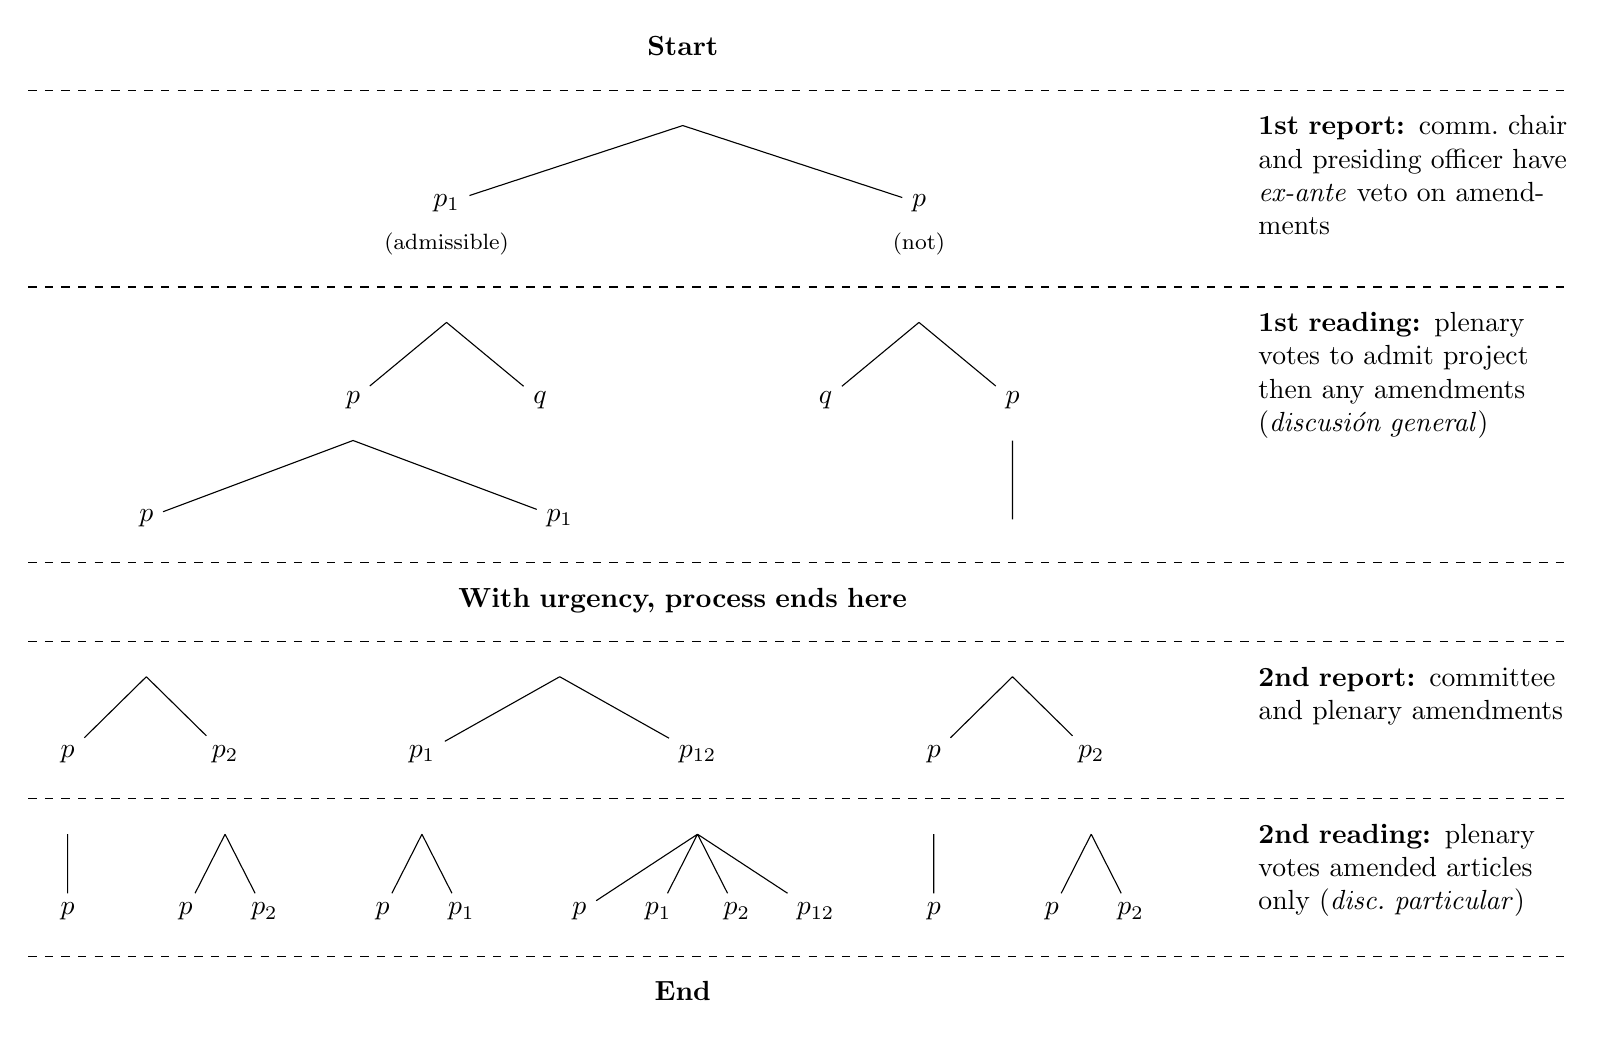
\begin{tikzpicture}
      \node[text width=10cm, text centered, anchor=north,fill=white] at (8.8125,-11) {\textbf{End}}; 
      %%%%%%%%%%%%%%%%%%%%%%%%%%%%%%%%%%%%%%%%%%%%%%%
      \draw[dashed] (0.5,-10.8) -- (20,-10.8);
      %%%%%%%%%%%%%%%%%%%%%%%%%%%%%%%%%%%%%%%%%%%%%%%
      \node[below] at (1,-10)    (o1)  {$p$}; 
      \node[below] at (2.5,-10)  (o2)  {$p$}; 
      \node[below] at (3.5,-10)  (o3)  {$p_2$}; 
      \node[below] at (5,-10)    (o4)  {$p$}; 
      \node[below] at (6,-10)    (o5)  {$p_1$}; 
      \node[below] at (7.5,-10)  (o6)  {$p$}; 
      \node[below] at (8.5,-10)  (o7)  {$p_1$}; 
      \node[below] at (9.5,-10)  (o8)  {$p_2$}; 
      \node[below] at (10.5,-10) (o9)  {$p_{12}$}; 
      \node[below] at (12,-10)   (o10) {$p$}; 
      \node[below] at (13.5,-10) (o11) {$p$}; 
      \node[below] at (14.5,-10) (o12) {$p_2$}; 
      \draw (1,-9.25) -- (o1)
            (3,-9.25) -- (o2)
            (3,-9.25) -- (o3)
            (5.5,-9.25) -- (o4)
            (5.5,-9.25) -- (o5)
            (9,-9.25) -- (o6)
            (9,-9.25) -- (o7)
            (9,-9.25) -- (o8)
            (9,-9.25) -- (o9)
            (12,-9.25) -- (o10)
            (14,-9.25) -- (o11)
            (14,-9.25) -- (o12);
      \draw[dashed] (0.5,-8.8) -- (20,-8.8);
      \node[text width=4cm, anchor=north west,fill=white] at (16,-9) {\textbf{2nd reading:} plenary votes amended articles only (\emph{disc.\ particular})}; 
      %%%%%%%%%%%%%%%%%%%%%%%%%%%%%%%%%%%%%%%%%%%%%%%
      \node[below] at (1,-8) (i21) {$p$}; 
      \node[below] at (3,-8) (i22) {$p_2$}; 
      \node[below] at (5.5,-8) (i23) {$p_1$}; 
      \node[below] at (9,-8) (i24) {$p_{12}$}; 
      \node[below] at (12,-8) (i25) {$p$}; 
      \node[below] at (14,-8) (i26) {$p_2$}; 
      \draw (2,-7.25) -- (i21)
            (2,-7.25) -- (i22)
            (7.25,-7.25) -- (i23)
            (7.25,-7.25) -- (i24)
            (13,-7.25) -- (i25)
            (13,-7.25) -- (i26);
      \draw[dashed] (0.5,-6.8) -- (20,-6.8);
      \node[text width=4cm, anchor=north west,fill=white] at (16,-7) {\textbf{2nd report:} committee and plenary amendments}; 
      % %%%%%%%%%%%%%%%%%%%%%%%%%%%%%%%%%%%%%%%%%%%%%%%
      \draw[dashed] (0.5,-5.8) -- (20,-5.8);
      \node[text width=10cm, text centered, anchor=north,fill=white] at (8.8125,-6) {\textbf{With urgency, process ends here}}; 
      %%%%%%%%%%%%%%%%%%%%%%%%%%%%%%%%%%%%%%%%%%%%%%%
      \node[below] at (2,-5) (g11) {$p$}; 
      \node[below] at (7.25,-5) (g12) {$p_1$}; 
      \node[below] at (4.625,-3.5) (g1) {$p$}; 
      \node[below] at (7,-3.5) (g2) {$q$}; 
      \node[below] at (13,-3.5) (g3) {$p$}; 
      \node[below] at (10.625,-3.5) (g4) {$q$}; 
      \draw (4.625,-4.25) -- (g11)
            (4.625,-4.25) -- (g12)
            (13,-4.25) -- (13,-5.25)
            (5.8125,-2.75) -- (g1)
            (5.8125,-2.75) -- (g2)
            (11.8125,-2.75) -- (g3)
            (11.8125,-2.75) -- (g4);
      \draw[dashed] (0.5,-2.3) -- (20,-2.3);
      \node[text width=4cm, anchor=north west,fill=white] at (16,-2.5) {\textbf{1st reading:} plenary votes to admit project then any amendments (\emph{discusión general})}; 
      %%%%%%%%%%%%%%%%%%%%%%%%%%%%%%%%%%%%%%%%%%%%%%%
      \node[below] at (5.8125,-1) (i11) {$p_1$}; 
      \node[text width=2cm, text centered] at (5.8125,-1.75) {\footnotesize{(admissible)}}; 
      \node[below] at (11.8125,-1) (i12) {$p$}; 
      \node[text width=2cm, text centered] at (11.8125,-1.75) {\footnotesize{(not)}}; 
      \draw (8.8125,-.25) -- (i11)
            (8.8125,-.25) -- (i12);
      \draw[dashed] (0.5,.2) -- (20,.2);
      \node[text width=4cm, anchor=north west,fill=white] at (16,0) {\textbf{1st report:} comm.\ chair and presiding officer have \emph{ex-ante} veto on amendments}; 
      %%%%%%%%%%%%%%%%%%%%%%%%%%%%%%%%%%%%%%%%%%%%%%%
      \node[text width=10cm, text centered, anchor=north,fill=white] at (8.8125,1) {\textbf{Start}}; 
      %%%%%%%%%%%%%%%%%%%%%%%%%%%%%%%%%%%%%%%%%%%%%%%
    \end{tikzpicture}  \\
\caption{Stylization of the voting agenda. Notation: $p$ is a project; $q$ the status quo; $p_1$, $p_2$, and $p_{12}$ are amendments, respectively to the first article, the second, or both. See text.}\label{f:agendaUrg}
\end{sidewaysfigure}

Notation eases exposition of Chile's legislative process. The three-article project is $p$, and $q$ the status quo (i.e., students and teachers get \$0 from this particular subsidy). Subindexing $p$ distinguishes versions with articles amended: $p_1$ with art.\ 1 amended, $p_2$ with art.\ 2 amended, and $p_{12}$ with both articles amended. Negotiation proceeds in four steps (schematized in Figure \ref{f:agendaUrg}).\footnote{See the C\'amara's standing rules (reglamento), especially arts.\ 118--189.} 

\begin{enumerate}
\item The question of amendment $p_1$'s admissibility into the \textbf{first report} starts it all. The choice is by the chamber's presiding officer, who has final authority to overturn the committee chair's earlier decision. Admitting $p_1$ substantially complicates down the tree. 
\item The bill's \textbf{first plenary reading} follows (rules call it \emph{discusi\'on general}). The question here is whether the full project should be admitted for consideration or not, ending the legislative process at the status quo: $p$ v. $q$. Next, a vote to also admit the amendment---if any---follows. Project $p_1$ (amendment admitted) or $p$ (not) is immeadiately referred back to committee for a second report. 
\item If the committee concurs with the floor, then the \textbf{second report} is the outcome of the first reading. But new amendments can be introduced, in committee or by private diputados (with one-third plenary backing). The committee chair and presiding officer can fail to admit these amendments too. For the sake of simplicity, the choice here is just on art.\ 2, although there are many other possibilities---different redefinitions, adding articles, or deleting them. When amended, the second report will be $p_2$ when the outcome of the first reading was $p$, and will be $p_{12}$ when it was $p_1$. 
\item The \textbf{second reading} proceeds one article at a time (\emph{discusi\'on particular}). Importantly, this excludes the subset of articles that were not amended/added/removed in previous steps. This subset (which may include every article if none were amended) is considered adopted with no plenary vote. Rejecting art.\ 1's amendment makes the project lose subindex 1; likewise with art.\ 2. So when $p_{12}$ is the second report, the plenary can accept one amendment, the other, both, or neither---as portrayed in the bottom row of Figure \ref{f:agendaUrg}. 
\end{enumerate}

An important element is how the process shortens when the proposal is declared urgent. The urgency is a form of restrictive procedure. When the executive issues a two week or act now message, \emph{the bill receives no second report} and both plenary readings occur at once. The key here is how urgencies preclude the second round of amendments. 

Had the presiding officer allowed $p_1$ in, plenary voting on its admissibility becomes the final vote on its adoption. At it most restrictive---when the presiding officer removed $p_1$---the plenary is presented with a take-it-or-leave-it urgent proposal $p$. The Chilean executive is therefore entitled to act as the Rules committee in the U.S.\ House, determining which bills receive a closed rule for plenary consideration. [Hay que regresar a ley org. y reglamento para ver si la caricatura es acertada]. 

Un perfil de preferencia para ilustrar podria ser el siguiente:
\begin{itemize}
\item La mayoría está cerca de los maestros y ordena las alternativas $p_{12}>p_{2}>p_{1}>p>q$ (de mejor a peor)
\item El gobierno:  $p>q>p_2>p_1>p_{12}$.
\end{itemize}


\section{Adaptaci\'on de Dion-Huber}

\begin{figure}
  \begin{center}
    \tikzstyle{mid}=[circle,draw]
    \begin{tikzpicture}
      % \node[rectangle,draw] (n) at (0,0) {Nature};
      %\node (n) at (0,0) {\footnotesize{(Nature): $\pi$}};
      \node[mid] at (2,0) (l) {\emph{C}};
      \node[mid] at (4,1) (e) {\emph{P}};
      \node[mid] at (6,0) (v) {\emph{F}};
      \node at (4,-1) (le) {$x_0$};
      \node at (6,2) (ee) {$x_F$};
      \node at (8,1) (ve1) {$x_C$};
      \node at (8,-1) (ve2) {$x_0$};
      % \node at (0,0.7) {\small{Strategies:}}; \node at (2,0.7)
      % {\footnotesize{---}}; \node at (4,0.7) {\footnotesize{$x^*$}};
      % \node at (6,0.7) {\footnotesize{$y^*(x)$}}; \node at (8,0.7)
      % {\footnotesize{$z^*(x)$}}; \node at (0,-1.7)
      % {\small{Outcomes:}};
      %\path[->] (n) edge (l);
      \path[-] (l) edge node [above, sloped]
      {\footnotesize{report}} (e) (e) edge node [below, sloped]
      {\footnotesize{urgent}} (v);
      % \path[] (n) edge node [below] {\footnotesize{$\pi$}} (l)
      \path[] (l) edge node [below, sloped] {\footnotesize{$x_C$}} (e);
      \path[-o] (l) edge node [below, sloped] {\footnotesize{not}} (le)
                (e) edge node [above, sloped] {\footnotesize{not}} (ee)
                (v) edge node [above, sloped] {\footnotesize{accept}} (ve1)
                    %edge node [above, sloped] {\footnotesize{over-}} (ve2)
                    edge node [below, sloped] {\footnotesize{reject}} (ve2);
    \end{tikzpicture}
    \caption{The game}\label{F:game}
  \end{center}
\end{figure}



\section{The received wisdom}

\begin{center}
\singlespacing
[U]rgency powers... can have dramatic effects on executive-legislative \\ 
relations, legislative organization, and the policy process more generally\\ 
---\citet[][:438]{morgenstern.2002b}
\end{center}
\onehalfspacing

%\citeauthor{carey.shugart.1998a}'s \citeyearpar{carey.shugart.1998a} monograph on executive unilateral powers does not discuss it. \citeauthor{londregan.2000a}'s \citeyearpar{londregan.2000a} study of legislative institutions in the Chilean Senate does not include the urgency authority in the index. 

\noindent Scholars have paid little attention to the urgency authority. \citeauthor{shugart.carey.1992}'s \citeyearpar{shugart.carey.1992} seminal monograph does not include it when computing the index of presidents' legislative powers. And while not addressing it directly either, \citeauthor{carey.shugart.1998a}'s \citeyearpar{carey.shugart.1998a} discussion of the delegation of unilateral authority to the executive offers clues of the logic behind the institution. Informational and valence asymmetries between Latin American executive and legislative branches create incentives for such delegation. Delays to reach agreement in assemblies offer further incentives by diminishing the value of policy \citep{baron.ferejohn.1989}, so rather than delegate proposal power within the chamber, legislators may find it preferable to let the president set the agenda. 

%\citet{siavelis.2002} is the first study to cover the urgency authority. He hypothesized urgencies' game-changer potential. His study of Chilean executive-legislative covers the first post-transition presidency revealed just how very frequently urgency messages were issued: slightly more than one-third of proposals in Congress received some form of urgency, and about 9 out of 10 of urgent bills were executive-initiated. Guided by semantics, analysis sought to discover if urgent bills, in fact, circulated the steps of the legislative process faster than the rest, and whether urgency status also increased the likelihood of bill passage. The study found mixed evidence. Among executive bills, consideration of urgent ones had somewhat shorter duration than the rest (medians of 134 and 160 days, respectively), but no palpable difference in success rates is appreciated (64 and 63 percent, respectively). 

\citet{siavelis.2002} is the only systematic study of the urgency authority we are aware of. Like Morgenstern's quote, he hypothesized the urgency power's game-changer potential. His study of Chilean executive-legislative in the first post-transition administration revealed the amazing frequency with which urgency messages were issued by President Aylwin: slightly more than one-third of proposals in Congress received some form of urgency, and about 9 out of 10 of urgent bills were executive-initiated. Guided by semantics, he also sought to discover if ``urgent'' bills, in fact, circulated the steps of the legislative process faster than the rest, and whether urgency status increased the likelihood of bill passage. The study found mixed evidence at best. Among executive bills, consideration of those urgent had somewhat shorter duration than the rest (medians of 134 and 160 days, respectively), but no palpable difference in success rates is appreciated (64 and 63 percent, respectively). 

The negative finding may bear relation to three elements. In their study of budgetary congressional oversight of the executive, \citet{berrios.gamboa.fiscChile.2006} warn against overstating the Chilean urgency authority's importance, as non-compliance entails no penalty for Congress---the next section develops this argument. While this may explain the lack of effects, it begs the question of why the president resorted so frequently to an authority that seems inconsequential. In other words, why make so many empty threats?

Another is a failure to control for urgency degrees---elaborated in section 3---in the analysis. \citeauthor{aleman.navia.UrgChi.2009}'s \citeyearpar{aleman.navia.UrgChi.2009} systematic study of executive success in Congress in three post-transition presidencies finds some of the evidence sought by Siavelis. Controlling for bill characteristics (such as key policy domains, the chamber where the bill originated, the government's seat margin, and presidential agenda size), urgency degrees had quite different effects in passage. Higher degrees significantly associate with better probability of executive success, but the lower made no statistical difference. Since, as will be seen, low-degree urgencies were much more prevalent, conflating them washes off the effect of the higher-degree. 

% longer review of aleman and navia
%\citeauthor{aleman.navia.UrgChi.2009}'s \citeyearpar{aleman.navia.UrgChi.2009} systematic study of executive success in Congress in three post-transition presidencies also inspects Chile's urgency authority. Among controls, their equation includes urgency authority usage in the right side. The unit is the individual bill, and the size of the executive agenda varies substantially over the years. Variation is quantitative  (Congress received about 150 presidential bills in each of the first 6 years after 1990, a numbrer that dropped to about 70 in the next 6 years, then climbed to about 100 in the final 4 years of their series) and qualitative, presidents manifesting different propensities to aim at constitutional reform. Of direct relevance are the findings on urgencies. Controlling for key policy domains, chamber of origin, seat margins, and presidential approval, and clustering errors by legislative year, different prioritization reveal quite different effects in passage. `Act now' and `2-week' notices significantly increased the probability of bill passage, but not `one month' notices. 

Finally, selection bias is an obstacle to measure urgency authority effects. Presidents, behaving strategically, are likely to target for urgency proposals that are markedly different from the rest in important ways, so the set of bills receiveing urgent status is not random. Like the Siavelis and Alem\'an-Navia studies, we recognize the endogeneity problem that arises but does not confront it methodologically. Until a more subtle identification design is proposed, findings must be taken with a grain of salt. The systematic study of the urgency authority in Chile that follows should contribute to pave the way to a solution. 

%If presidents, behaving strategically, were to target for urgency proposals that are markedly different from the rest in important ways, a problem of endogeneity arises. Classify proposals based on how difficult passage is expected: easy, hard, and impossible. If left on their own, the easy proposals would be approved faster, the hard slower, the impossible never. A strategic president should concentrate the urgency authority in the hard group, leaving easy proposals mostly on their own, while abandoning the hopeless group of impossible proposals, that will not be observed. As a consequence, comparing

%The relevant quantity of interest is whether the use of the urgency authority affects bill passage (success, speed, amendments, and so forth) compared to the same bill with no urgency attached. The fundamental problem of causal inference is immediately evident. The executive presumably targets bills for urgency strategically, so that the selection mechanism cannot be assumed random. If, for example, more complex and divisive legislation takes longer, is likelier to fail and likelier to be tagged urgent, separating effects requires more subtle methods than used up to now.


\section{Costly scheduling and inaction}

Five constitutions of the Americas give executives power to interfere, to some degree, with the assembly's voting schedule \citep{morgenstern.2002b}. The urgency authority varies considerably. In Brazil, the assembly must act on a bill deemed urgent withing 45 days, or else it takes precedence over legislative business. The president can declare any executive-initiated bill urgent at any time. And, since 2001, all executive unilateral policy (\emph{medidas provis\'orias}) become urgent bills upon publication. In Colombia, urgent bills go to the top of the voting schedule immediately. In Uruguay and Chile, legislators must act within a pre-specified, short period. Failure to do so converts the urgent bill into law in Uruguay, although three-fifths of any chamber's membership can remove the project's urgent status. As said, in Chile the consequences of inaction are indetermined. And in Mexico since 2012, the president can propose up to two bills with urgent at the start of each biannual sessions period, which must scheduled for floor consideration within 30 days. As in Chile, how to proceed in case of legislative non-compliance is indetermined.\footnote{Constitutional articles enshrining this authority are the following: Brazil 62 and 64; Chile 74; Colombia 163; Mexico 71; and Uruguay 168.7.}

%\emm{How does this compare with extra-ordinary sessions? Some presidents can summon legislators to a special session to discuss, exclusively, a specific bill defined ex-ante. Limits? If few, might resemble urgency authority... Check}

\begin{figure}
  \centering
    \tikzstyle{mid}=[circle,draw]
    \begin{tikzpicture}
      \node[mid] at (2,-.5) (e) {\emph{E}}; 
      \node[mid] at (4,1) (l) {\emph{L}}; 
      \node[right] at (4,-2) (ee) {$x_0+o$}; 
      \node[right] at (6, 2.5) (le1) {$x_1$};  
      \node[right] at (6, 1) (le3) {$x_0-c$}; 
      \node[right] at (6,-.5) (le2) {$r+o-k$}; 
      \path[-]  (e) edge node [above, sloped] {\footnotesize{propose}} (l);
      \path[]   (e) edge node [below, sloped] {\footnotesize{$x_1$}}   (l); 
      \path[-o] (e) edge node [below, sloped] {\footnotesize{not}}     (ee) 
                 (l) edge node [above, sloped] {\footnotesize{accept}} (le1) 
                 (l) edge node [below, sloped] {\footnotesize{ignore}} (le2);
      \path[-o] (l) edge node [above, sloped] {\footnotesize{reject}} (le3);
    \end{tikzpicture}  \\
 \footnotesize{
 \begin{tabular}{lrrr}
  Case                       & $r$   & $c$   & $k$      \\ \hline
  Chile                      & $x_0$ & 0     & $\geq0$     \\
  Brazil (urgency), Colombia & $x_0$ & 0     & $\geq o$    \\
  Brazil (MPs)               & $x_0$ & $>0$  & $\geq o$    \\
  Brazil (MPs up to 2001)    & $x_1$ & $>0$  & 0        \\
  Mexico (4 bills yearly)    & $x_0$ & 0     & ?        \\
  Uruguay                    & $x_1$ & 0     & 0        \\
  \end{tabular}
  }
\caption{Urgency authority and costly scheduling and rejections}\label{f:costly}
\end{figure}

Figure \ref{f:costly} extends the framework used throughout the book to ease the comparison of different urgency authorities. Key in the stylization is that rejection of undesirable executive proposals is costly for the assembly. The framework reveals similarities and differences between urgency authorities, and consequences for executive-legislative bargaining. It is set as a two-player game between the executive and the pivotal legislator. The former starts by proposing urgent policy $x_1$, or ending the game with the status quo $x_0$ unchanged. Terminal nodes in the game tree indicate the policy outcome ($x_0$, $x_1$, or $r$) and associated costs (all elaborated below). Costs are all borne by the legislator, whose payoff is the value of the policy outcome indicated and the value of the costs: in the case of the bottom terminal node, for instance, this would be $u_l(x_0)+o$ (where $u_l$ is Euclidian utility). 

Given scarce committee and plenary time, scheduling anything for consideration entails an opportunity cost $o$. Conceptually, $o$ is the value of the best alternative policy that the legislator might adopt if scheduled instead of proposal $x_1$. With an institution that no two (or more) proposals are scheduled simultaneously, considering $x_1$ inevitably postpones the consideration of the best alternative---indefinitely, perhaps, since the agreement to schedule it next may break down \citep{cameron.2000,wawro.schickler.filibuster.2007}. So, when no proposal is made, value $o$ can be realized by the legislator in the bottom terminal node (he is free to schedule the alternative), adding up to the policy payoff. 

If called to play, the legislator faces three actions to choose from, all leading to terminal nodes. For ease of exposition, costs other than $o$ are initially set to zero ($c = k = 0$), cancelling out of the description. The restriction is relaxed afterwards. The legislator can accept the proposal, replacing the status quo with policy at $x_1$. The legislator could alternatively retain the status quo by rejecting the proposal. Both choices entail an opportunity cost due to the need to schedule the bill for acceptance or rejection. And the legislator could opt to ignore the proposal, policy reverting to a pre-defined reversion outcome $r$. Unlike the other alternatives, ignoring frees legislative time to schedule something else, and $o$ adds to the value of the outcome. 

% Mex: exec-init actually rejected (diputados Weldon)
% 58 none
% 59 4 down (3 negative reports, 1 voted)
% 60 4 down (2 negative reports, 2 voted) (both voted and 1 report were carry-overs from Fox's)
% 61 2 down (1 negative report, 1 voted) (report was carry-over from Fox's) (preclusión adopted here: after 45-90 days with no report, Mesa can archivar proposals... a bunch were precluidas en bloc)
%
% Mex: exec-init passed (diputados Weldon, includes minutas)
% 2000-01 21
% 2001-02 30
% 2002-03 29
% 2003-04 16
% 2004-05 32
% 2005-06 23
% 2006-07 15
%
% Mex: ex-init (diputados infosil, excludes minutas and carryovers)
% 58: 63 in, 55 approved
% 59: 49 in, 31 approved
% 60: 42 in, 38 approved
% 61: 32 in, 26 approved
%
% Synthesis of Weldon/Infosil data
% 58:  63 in,  55 approved, 0 rejected,  8 ignored
% 59:  49 in,  31 approved, 4 rejected, 14 ignored
% 60:  42 in,  38 approved, 1 rejected,  3 ignored 
% 61:  32 in,  26 approved, 1 rejected,  5 ignored
% all:186 in, 150 approved, 6 rejected, 30 ignored
%
%          period       exec-init   rechazadas  retiradas  aprobadas pendientes
% Chile    1998-2014      1469                113            1075       281
% Br       1995-2010      1650          73         109       1100       367
% Urug     1995-2005      1050                                709
% Urug     1985-1990       416                                269
% Urug     1985-2000      1456                                965

% \begin{table}
% \centering
% \begin{tabular}{lcrrrrr}
% Case   & Period     & Withdrawn & Rejected & Pending & Total & (N) \\ \hline
% Brazil & 1995--2010 &  13       &   20     &   67    &  100  & (549) \\
% Chile  & 1998--2014 & \mc{2}{c}{29}        &   71    &  100  & (394) \\
% Mexico & 2000--2012 &   0       &   17     &   83    &  100  &  (36) \\
% \end{tabular}
% \caption{How executive bills failed in three cases. Sources: Mexican executive bill approval is from \protect\url{http://sil.gobernacion.gob.mx}, rejections kindly shared by Jeff Weldon. Gobernaci\'on reports carry-over bills from previous Legislaturas in a residual category, and some bills ignored by the current Legislatura were in fact considered by subsequent ones in the period. Of these, 4 more were actually rejected (3 by negative report, 1 by floor vote).}\label{t:exBillFail}
% \end{table}

Reversionary policy $r$ varies across constitutions. The Uruguayan reverts policy to executive proposals declared urgent but not scheduled for a vote ($r=x_1$). The Brazilian also did in cases of unscheduled urgency by \emph{medida provis\'oria} up to 2001, when the constitution was amended.\footnote{\emph{Medidas provis\'orias} expire 60 days after publication. Before the reform, a Supreme Court ruling legalized the option of re-issuing MPs that had not been discussed and voted in Congress upon expiration, leading to the instituion described in the text ($r=x_1$). The reform adopted 9/11/2001 limits presidents to one MP re-issue, with migration to the top of the voting schedule in case of congressional inaction. See \citet{figueiredo.etal.1996}.} The rest, including Brazil since 2001, revert to the status quo ante ($r=x_0$). Absent costs other than $o$ (and leaving aside the possibility of $o<0$), ignoring undesirable proposals dominates rejecting them, foregoing opportunity costs. This jibes with evidence of assemblies brushing aside undesired executive proposals by inaction rather than actual rejection.\footnote{Executive bills that failed to pass in three legislatures overwhelmingly remained pending, as opposed to explicitly rejected or withdrawn. Of 549 failed executive bills in Brazil between 1995 and 2010, 67 percent remained pending; of 394 in Chile between 1998 and 2014, 71 percent remained so; and of 36 in Mexico between 2000 and 2012, 83 percent did. The highest rate in Mexico coincides with the most limited urgency authority, and lowest in Brazil with the least limited. Sources: Brazilian and Chilean data from databases in this and next chapters, Mexican executive bill approval is from \protect\url{http://sil.gobernacion.gob.mx}, rejections kindly shared by Jeff Weldon.} The alternative reversion policy $r=x_1$ brings a drastic change in executive-legislative relations, as congressional inaction becomes a way of adopting urgent presidential policy more cheaply than through actual approval.

Relaxing the nil costs restriction brings further depth into the comparative framework. Cost $c>0$ lowers the legislator's status quo value after rejection of the proposal. This cost is relevant for Brazil only, and is elaborated elsewhere. Suffice to say here that Brazil since 2001 conflates the urgency authority with executive unilateral power, and cost $c$ is related to the latter only---arising from the difference in turning down policy recently set in motion and turning down a policy prospect. 

% USE FOR BRAZILIAN CHAPTER: Cost $c$ is associated with unilateralism per se, independent of the urgency authority, and therefore is applicable to the Brazilian case only (where both institutions are compounded since 2001). \emph{Medidas provis\'orias} are presidential decrees with immediate force of law, and unlike statutory proposals, they turn potential into actual winners and losers before the assembly votes on them. At the statutory proposal stage, there is an expectation that a group might receive a flow of benefits if all goes according to plan. A fair amount of uncertainty surrounds all, both about the likelihood that policy will in fact materialize and about the size and scope of benefits associated with the details of the policy that eventually passes. Once adopted, however, this uncertainty vanishes. When policy is adopted unilaterally, winners and losers are clearly identified before the measure is discussed and voted, changing the obstacles that the assembly may face. Rescinding the decree will imply surmounting an identifiable opposition that could organize more cheaply than the diffuse kind \citep{olson.1965} anticipating policy by statute. This translates into cost $c>0$. % Add that, when devising policy, desirable to concentrate benefits (and claim credit) while diffusing costs.  

Cost $k>0$ mitigates, or even cancels, the value of the opportunity cost realized by ignoring the president's proposal. It arises from issue salience and what \citet{neustadt.1990} called the president's power to persuade. Raising urgency conveys a sense of importance and of imperative immediate attention. By signaling presidential priority, coupled with a clever communication strategy, the urgency authority may place issues in the public agenda, increase media attention, and nurture public debate. An undesired proposal that could have easily been dusted under the carpet in normal circumstances will, as a consequence of increased salience, be harder to duck---adding a cost $k>0$. And salience aside, cost $k$ is magnified when the institution brings an urgent but unconsidered proposal to the top of the assembly's Day's Order, as in Colombia and Brazil. In both cases, constitutions establish a reversion schedule for legislative inaction: consider the urgent proposal, or nothing. At this point, continuing to postpone proposal $x_1$ subtracts value $o$ once for every additional session until the proposal is considered, resulting in $k>o$. 

The table accompanying Figure \ref{f:costly}'s game tree summarizes costs associated with rejection and ignoring urgent proposals in the five constitutions. Cost $c>0$ is Brazil specific. Urgency non-compliance being the same as tacit acceptance when $r=x_1$, a zero cost is associated ($k=0$). And reversion schedule pulling the urgent proposal to the top imply non-compliance costs more than offsetting the gains of an opportunity cost foregone ($k>o$). In Mexico, the consequences of inaction remain indeterminate. 

\newcommand\mygt{\mathrel{\stackrel{\makebox[0pt]{\mbox{\normalfont\footnotesize ?}}}{>}}} % greater than sign with question mark on top

And key for our paper is whether or not non-compliance costs different from zero arise in Chile and are large enough to offset opportunity costs ($k \mygt o$). Failure to offset in the framework developped leaves the president's urgency as an inconsequential authority, as the next section demonstrates. %Evidence below does not estimate cost $k$, but it show patterns consistent with $k>o$ at least part of the time or over a subset of proposals.  

\section{Variable urgency degrees}
\begin{center}
Presidential power is the power to persuade ---Neustadt\footnote{\citet[][11]{neustadt.1990}}
\end{center}

The constitution (art.\ 74) stipulates that the president can urge action on any bill (not just executive proposals) at any stage of the legislative process. The chamber receiving the urgency message is compelled to ``discuss and vote'' the bill before a deadline. The exception are urgency messages raised over bills in conference committee to resolve inter-cameral differences, requiring timely action from the conference and then each individual chamber.

The congressional organic law (arts.\ 26 and 27) defines the breadth of the interference, giving the president a choice of sending `one month' (\emph{urgencia simple} or 30 days), `two week' (\emph{urgencia suma} or 15 days), or `act now' (\emph{discusión inmediata} or 6 days) notices. The organic law was amended in July 2010, four months into the newly elected Legislature and concurrent presidential administration, substantially relaxing the deadlines for the `act now' and `two week' urgencies, originally set at 10 and 3 days, respectively. `One month' urgencies remained unchanged. Issuing maximal urgency in the right circumstances---an act-now message attached to a bill in conference before 2010---gave each instance just one day to act: one for the conference to report a compromise bill, and one for each chamber to sequentially consider and push the bill to the floor for a vote (congressional practice is well summarized by the library of Congress at \url{http://www.bcn.cl/ecivica/formacion/}.) The president may remove the urgency at will, with immediate effects. Urgency messages expire at the end of the ordinary period on March 10th every year. 

The constitution, it must be noted, sets only a floor for the urgency authority, defining one month urgency only. Higher degrees are set by the organic law. High-degree urgency is therefore vulnerable to congressional majorities, who might be inclined to relax the deadlines available if that were in their interest---as, in fact, was done in 2010. But the constitution (art.~66) also raises the bar for this by requiring the vote of four-sevenths ($\approx 57$ percent) of each chamber's membership for organic law passage and amendment. While below the two-thirds membership needed for constitutional reform, no coalition has exceeded the organic law threshold in both chambers since the return to democracy.

Vagueness surrounds key aspects of the urgency authority. When a 30-day limit is set, for instance, no indication is given of whether those are calendar, business, or session days. I treat the messages in weeks rather than days given imprecision (and, when coding deadlines in the empirical sections below, arbitrarily rely on business days). More important, no formal reversionary course of action is defined, and no hint of rulings by the Constitutional Tribunal filling in the institutional void could be found. As seen in the previous section, I interpret indeterminacy as reversion to the status quo with no effect on the voting schedule.

In the absence of a formal penalty for inaction---like Uruguayan reversion to $x_1$, or placing Brazilian legislative business on hold until the urgency is heeded---only a sizeable cost $k$ remains to prevent the Chilean assembly ignoring executive proposals: unless $k>o$, ignoring dominates rejecting an undesirable proposal. Like vetoes, explicit rejections can have position taking value, as shown in chapter \ref{ch:posModel}. And cost $k$ may be key to remove (or, at least, minimize) executive disadvantage in the presence of opportunity costs. 

\begin{figure}
  \centering
\begin{tabular}{c|c}
   Chile & Uruguay \\
    \tikzstyle{mid}=[circle,draw]
    \begin{tikzpicture}[scale=0.7]
      \node[mid] at (2,-.5) (e) {\emph{E}}; 
      \node[mid] at (4,1) (l) {\emph{L}}; 
      \node[right] at (4,-2) (ee) {$x_0+o$}; 
      \node[right] at (6, 2.5) (le1) {$x_1$};  
      \node[right] at (6, 1) (le3) {$x_0$}; 
      \node[right] at (6,-.5) (le2) {$x_0+o-k$}; 
      \path[-]  (e) edge node [above, sloped] {\footnotesize{prop.}} (l);
      %\path[]   (e) edge node [below, sloped] {\footnotesize{$x_1$}}   (l); 
      \path[-o] (e) edge node [below, sloped] {\footnotesize{not}}     (ee) 
                 (l) edge node [above, sloped] {\footnotesize{acc.}} (le1) 
                 (l) edge node [below, sloped] {\footnotesize{ign.}} (le2);
      \path[-o] (l) edge node [above, sloped] {\footnotesize{rej.}} (le3);
    \end{tikzpicture}
         &
    \tikzstyle{mid}=[circle,draw]
    \begin{tikzpicture}[scale=0.7]
      \node[mid] at (2,-.5) (e) {\emph{E}}; 
      \node[mid] at (4,1) (l) {\emph{L}}; 
      \node[right] at (4,-2) (ee) {$x_0+o$}; 
      \node[right] at (6, 2.5) (le1) {$x_1$};  
      \node[right] at (6, 1) (le3) {$x_0$}; 
      \node[right] at (6,-.5) (le2) {$x_1+o$}; 
      \path[-]  (e) edge node [above, sloped] {\footnotesize{prop.}} (l);
      %\path[]   (e) edge node [below, sloped] {\footnotesize{$x_1$}}   (l); 
      \path[-o] (e) edge node [below, sloped] {\footnotesize{not}}     (ee) 
                 (l) edge node [above, sloped] {\footnotesize{acc.}} (le1) 
                 (l) edge node [below, sloped] {\footnotesize{ign.}} (le2);
      \path[-o] (l) edge node [above, sloped] {\footnotesize{rej.}} (le3);
    \end{tikzpicture}
         \\
  \mc{1}{l|}{Case 1: $k<o$} & \mc{1}{l}{Case 3: $k \equiv 0$} \\
          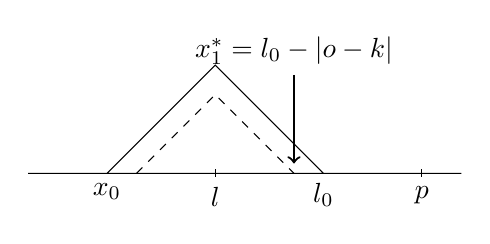
\begin{tikzpicture}[scale=0.5]
          \draw (0,0) -- (11,0) 
          (2,0) node[below] {$x_0$} -- (4.75,2.75) -- (7.5,0) node[below] {$l_0$}; 
          \draw[dashed] 
          (2.75,0) -- (4.75,2) -- (6.75,0); 
          \draw (4.75,0.1) -- (4.75,-0.1) node[below] {$l$}
                (10,0.1) -- (10,-0.1) node[below] {$p$};
          % \draw[->] 
          %       (7,-1) node[below] {$(l_0+o)$} -- (7,-0.25);
          \draw[->, thick] 
                (6.75,2.5) node[above] {\textbf{$x_1^*=l_0-|o-k|$}} -- (6.75,0.25);
        \end{tikzpicture}
         &
        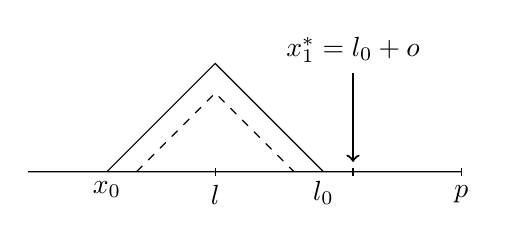
\begin{tikzpicture}[scale=0.5]
          \draw (0,0) -- (11,0) 
          (2,0) node[below] {$x_0$} -- (4.75,2.75) -- (7.5,0) node[below] {$l_0$}; 
          \draw[dashed] 
          (2.75,0) -- (4.75,2) -- (6.75,0); 
          \draw (4.75,0.1) -- (4.75,-0.1) node[below] {$l$}
                (11,0.1) -- (11,-0.1) node[below] {$p$}
                (8.25,0.1) -- (8.25,-0.1) ;
          % \draw[->] 
          %       (8,-1) node[below] {$(l_0-o)$} -- (8,-0.25);
          \draw[->, thick] 
                (8.25,2.5) node[above] {\textbf{$x_1^*=l_0+o$}} -- (8.25,0.25);
        \end{tikzpicture}
         \\
  \mc{1}{l|}{Case 2: $k \geq o$} &  \\
        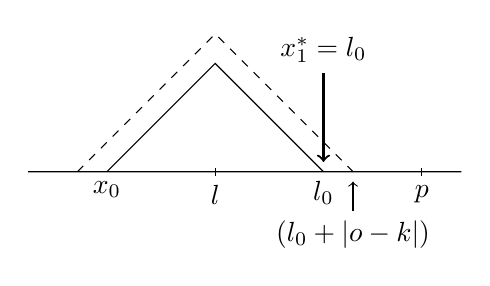
\begin{tikzpicture}[scale=0.5]
          \draw (0,0) -- (11,0) 
          (2,0) node[below] {$x_0$} -- (4.75,2.75) -- (7.5,0) node[below] {$l_0$}; 
          \draw[dashed] 
          (1.25,0) -- (4.75,3.5) -- (8.25,0); 
          \draw (4.75,0.1) -- (4.75,-0.1) node[below] {$l$}
                (10,0.1) -- (10,-0.1) node[below] {$p$};
          \draw[->] 
                (8.25,-1) node[below] {$(l_0+|o-k|)$} -- (8.25,-0.25);
          \draw[->, thick] 
                (7.5,2.5) node[above] {\textbf{$x_1^*=l_0$}} -- (7.5,0.25);
        \end{tikzpicture}
         &
         \\
       \end{tabular}
\caption{Equilibrium costly-scheduling proposals in three cases}\label{f:chiUruEql}
\end{figure}

To see this, I contrast Chilean and Uruguayan versions of the game in Figure \ref{f:chiUruEql}, revealing how the size of $k$ relative to $o$ and the reversion point determine who is advantaged by the urgency authority. The Chilean institution, in the left panel, operates identically with or without an urgency message---although cost $k$ may not arise without urgency, as will be seen. The Uruguayan institution, in the right, necessitates an urgent presidential proposal, or else the $r=x_1$ reversion does not kick in abd the game is identical to Chile's. Proceeding backwards, the Chilean legislator compares relative utilities $u_l(x_1)$, $u_l(x_0)$, and $u_l(x_0)+o-k$. With $x_0$ and costs $o$ and $k$ set exogenously, a baseline for the optimal reaction to the president's proposal can be derived. Giving players specific preferences relative to a status quo aides in seeing the bargaining logic and institutional effects. An interesting example, with room for inter-branch compromise in policy, is $x_0 < l < p$, analyzed graphically below the game tree in the figure. (I do not derive the full equilibrium, which is in line with the model in chapter \ref{ch:posModel}.) Using the book's standard notation and spatial payoffs, $l_0$ in the figure is policy leaving the legislator indifferent to the status quo (before netting any costs). If ignoring leaves the status quo intact, it also adds $o-k$ to the legislator's utility, and the net value of ignoring must therefore be read through the dashed indifference sets. Whenever the ignoring cost less than counters the opportunity cost (i.e., $k<o \iff o-k>0$, as in the figure's case 1), the dashed-line indifference set falls inside the limits of the standard indifference set and ignoring gives a bonus, dominating rejecting. When the president calibrates a proposal at $x_1 = l_0$---which, in the standard game, prompts acceptance---the legislator is better off ignoring it (thus receiving $x_0$ at the dashed value, which is closer to ideal point $l$ than the accepted proposal's value). Acceptance requires further presidential concessions: a proposal at $x_1=l_0-(-k+o)$ leaves the legislator indifferent, and is accepted.\footnote{This claim assumes that, when indifferent between accepting and not, the legislator accepts. Locating the proposal a tiny $\epsilon$ closer to the ideal, as in chapter \ref{ch:posModel}, achieves the same without this assumption, but is less economical in notation.} 

When $k\geq o \iff o-k\leq0$ (as in case 2), the dashed line falls beyond the limits of the legislator's costless indifference set, and now rejecting dominates ignoring. In which case a proposal at $x_1=l_0$ yields identical payoff to the status quo and is accepted, as in the standard game. And in case 3, where only cost $o$ intervenes (and is assumed positive), ignoring dominates accepting, leaving the executive room to extract welfare from the legislator. Ignoring a proposal at $x_1=l_0$, valued with the dashed line (which, given $o>0$, is within the limits of the costless indifference set), dominates both accepting and rejecting. With that in mind, an alternative proposal at $x_1=l_0+o$, leaving the legislator indifferent, is also ignored (tacitly accepted) but with fewer executive concessions. 

In sum, Uruguayan reversion to the urgent proposal always operates in favor of the executive, who gains policy influence directly proportional to the size of opportunity cost $o$. In contrast, Chilean reversion to the status quo can operate against executive influence. When the cost legislators pay for ignoring executive proposals cannot offset the opportunity cost of finite scheduling time, the legislator gains influence inversely proportional to $|o-k|$. Executive-legislative influence is re-balanced in Chilean-type urgency only when cost $k$ is large enough to compensate the legislator's opportunity cost. 

It is worthwhile to elaborate on two routes towards fulfillment of the balancing condition $o<k$: by lowering opportunity cost $o$ relative to ignoring cost $k$, or by increasing $k$ relative to $o$. Proposing genuine policy priorities---that is, labeling urgent an objectively urgent issue---drops the size of $o$. Given that genuine priorities are rare, if this were the only route then urgency messages would be rare, something that the Chilean evidence contradicts. The second route therefore seems more attractive. How can presidents increase the size of cost $k$?

\citeauthor{neustadt.1990}'s \citeyearpar{neustadt.1990} study of the modern U.S.\ presidency offers elements connecting the urgency, and especially the president's qualification of the urgency, with the size of cost $k$. Urgency communicates presidential priority \citep{aleman.navia.UrgChi.2009}, a message that legislators may disregard, postponing the proposal's consideration. If no perils are in sight, legislators can safely choose to ignore the message, postponing the proposal's consideration. But, with the president involved, perils are likely, and legislators will need to quantify expected damages. ``With hardly an exception, those who share in governing [under separation of power] are aware that at some time, in some degree, the doing of \emph{their} jobs, the furthering of \emph{their} ambitions, may depend on the President... Their need or fear is his advantage'' (31, emphasis in original). Coupled with a clever communication strategy prompting vivid stories that illustrate and personalize national problems (what Neustadt calls happenings), the urgency can mobilize public opinion favorably for the issue \citep{iyengar.kinderNewsMatter1987}. Ignoring the proposal becomes costly. So, all else equal, a `two week' notice has a larger $k$ (or, at least, never lower) than a `one month, and an `act now' message has a larger $k$ (or, at least, never lower) than either other. 

%Urgency type frequency, in fact, reveals a tendency to rely less often on more urgent messages (descriptive data is presented in the next section). `Act now' notices were roughly 3 to 5 times less frequent than `two week' ones in a recent 16-year period. The frequency differential between `two week' and `one month' notices is less sharp, but a tendency is distinguishable. 

%This observation dovetails with previous characterizations of the Chilean urgency authority. \citet{berrios.gamboa.fiscChile.2006} advance the notion that, in spite of reversion $r=x_0$, the assembly may indeed face political costs of ignoring urgency messages on salient proposals. 

%This leads to another puzzle: Why are `one month' messages so numerous?\footnote{Quoting a former legal chief of staff at the Presidency, \citeauthor{berrios.gamboa.fiscChile.2006} describe `one month' notices as ``merely symbolic, exerting no real pressure on Congress'' (p.~117). Likewise, \citet{aleman.navia.UrgChi.2009} see low-degree urgency as ``signals of presidential attention'' (p.~404). Suggests that non-compliance should be concentrated in this category, this can be verified.} 

\section{The data}

\begin{table}
\begin{center}
\begin{tabular}{lrrrr}
List        & 1998--2002    & 2002--06 & 2006--10 & 2010--14 \\ \hline
\mc{5}{l}{\emph{~~C\'amara de Diputados}} \\
President's & 58            & 53       & 51       & 50       \\
Opposition  & 42            & 48       & 47       & 48       \\
Regional    &               &          & 3        & 2        \\ \hdashline
Total       & 100           & 100      & 100      & 100      \\ \hline
\mc{5}{l}{\emph{~~Senate}} \\
President's & 50            & 50       & 55       & 45       \\
Opposition  & 50            & 50       & 45       & 55       \\ \hdashline
Total       & $100^{\dagger}$ & 100      & 100      & 100      \\ \hline
\mc{5}{r}{\footnotesize{$^\dagger$vacant seats dropped}}
\end{tabular}
% \begin{tabular}{lrrrrrr}
% Coalition   & 1990--94 & 1994--98 & 1998--2002    & 2002--06 & 2006--10 & 2010--14 \\ \hline
% \mc{7}{l}{\emph{~~C\'amara de Diputados}} \\
% President's & 60       & 58       & 58            & 53       & 51       & 50       \\
% Opposition  & 40       & 42       & 42            & 48       & 47       & 48       \\
% Regional    &          &          &               &          & 3        & 2        \\ \hdashline
% Total       & 100      & 100      & 100           & 100      & 100      & 100      \\ \hline
% \mc{7}{l}{\emph{~~Senate}} \\
% President's & 48       & 46       & 50            & 50       & 55       & 45       \\
% Opposition  & 52       & 54       & 50            & 50       & 45       & 55       \\ \hdashline
% Total       & $100^*$  & $100^*$  & $100^{*\dagger}$ & 100      & 100      & 100      \\ \hline
% \mc{7}{l}{\footnotesize{Notes: $^*$ vacant seats dropped; $^\dagger$ margin varied above and below 50/50 due to vacancies.}}
% \end{tabular}
\caption{The president's status in Congress. Percent seats controlled by electoral lists in each chamber. The president's list in 1998--2010 was Concertaci\'on; it was Alianza afterwards. Regional list includes major-list splinters (from Christian Democrats and UDI). President's status in the Senate slightly and briefly oscilated above and below majority due to vacant seats. Source: prepared with information from \protect\url{www.camara.cl}.}\label{t:congressSeats}
\end{center}
\end{table}

Original data was collected to investigate the urgency authority in Chile. The C\'amara de Diputados' web page (\url{www.camara.cl}) was scraped in November 2014 in search for the record (\emph{bolet\'in}) of every proposal made between 11 March 1998 and 10 March 2014, inclusive.\footnote{Queries were sent to the congressional staff in October 2014 about the existence of an official API or FTP site where this well-structured data could be downloaded en bloc. There was no response, so an automated script was prepared to retrieve the information directly. The C\'amara's web page is javascript-rich, an obstacle surmounted with \texttt{Python}'s Selenium library, putting together the bits and pieces of the scraping process. A commented version of the script and the dataset will be posted online upon publication. Data analysis was done with a multiplicity of \texttt{R}'s libraries.} Years before 1998 antedate Internet publication and were dropped, as data completeness in the primary source remains to be verified. The period selected fully covers two Senates, four C\'amaras, and three presidencies (plus the last two years of an earlier presidency). 

The span offers variance in the size and status of the president's coalition in Congress. Given electoral list voting unity since the return to democracy \citep{carey.2002,aleman.saieg.coalUnityChile.2007}, the seats they control are a good indicator of the executive's legislative support. As Table \ref{t:congressSeats} reports, the president's coalition was always in control of the C\'amara, but has controlled Senate majorities between 2006 and 2010 only (coinciding with the first Bachelet administration). By requiring 67, 60, and 57 percent votes of each chamber, respectively, constitutional reform, constitution-interpreting legislation, and organic laws therefore always required votes across the aisle. 

The source publishes detailed reports with the general traits of legislation: who proposed the bill, when, in what chamber, what it deals with, its status at the time of consultation, and so forth. The report also lists and dates the proposal's milestones in the bicameral legislative process: committee referrals, reports to the plenary, floor discussion and voting, navette to the other chamber, and more. Of direct relevance, all urgency messages received by the chambers are listed chronologically. All this information was systematized.

% verify numbers in chillBill.r (above xtable command)
\begin{table}
\centering
\begin{tabular}{lrrr}
                                &  by           &  by          &    by      \\
Bills                           &  legislators  &  president   &    ~~~~either  \\ \hline
introduced                      &        5,526  &       1,461  &     6,987  \\
as \%                           &    \emph{79}  &   \emph{21}  & \emph{100} \\ \hdashline
passed                          &          404  &       1,059  &     1,463  \\
as \%                           &    \emph{28}  &   \emph{72}  & \emph{100} \\
as \% of introduced             &     \emph{7}  &   \emph{72}  &  \emph{21} \\ \hdashline
declared urgent (once at least) &          349  &       1,013  &     1,362  \\
as \%                           &    \emph{26}  &   \emph{74}  & \emph{100} \\
as \% of introduced             &     \emph{6}  &   \emph{69}  &  \emph{19} \\ \hdashline
declared urgent \& passed       &          167  &         759  &       926  \\
as \%                           &    \emph{18}  &   \emph{82}  & \emph{100} \\
as \% of declared urgent        &    \emph{48}  &   \emph{75}  &  \emph{68} \\ \hline
\end{tabular}
\caption{Proposals, legislation, and the urgency authority 1998--2014}\label{T:billDescriptives}
\end{table}

Table \ref{T:billDescriptives} offers a general summary of bill introduction, passage, and urgency incidence in the period. Nearly seven thousand pieces of legislation were proposed, 412 yearly on average. Most introduction was by members of Congress, who made four proposals for every bill by the president (79 vs.\ 21 percent). In terms of success rates, however, the branch ratio inverts, a member turning one proposal into law for every three by a president (27 vs.\ 73 percent). And while members' success rate was dismal (7 percent), they still managed to add about four hundred statutes in the period due to the sheer volume of proposals made. 

It is striking that one proposal in five was urgent. The 1,362 bills deemed urgent at some point in the legislative process attest to a permissive notion of urgency by Chilean presidents. Also note the close similarity of relative figures in the second (urgency) and third (passed bills) groups of table rows. The large overlap of the urgent bills and bills passed subsets suggests, coincident with \citet{aleman.navia.UrgChi.2009}, that urgency and success correlate strongly: the passage rate of members' bills declared urgent skyrocketed to 48 percent, up from 7 percent altogether (the difference is small for executive bills). But concluding that urgency improves bills' odds misses that the reverse is also possible, proposals with better prospects in Congress strategically receiving the bulk of urgency messages---the problem of selection bias discussed above \citep[cf.][]{jacobson.kernell.1983}. 

% latex table generated in R 3.1.2 by xtable 1.7-4 package
% Wed Feb 4 17:24:48 2015
\begin{table}
\centering
\begin{tabular}{rrrrr|r}
      & 1998--2002 & 2002--06 & 2006--10 & 2010--14 & 1998--2014 \\ \hline
 \multicolumn{5}{c|}{\textbf{Part A. Individual messages}} \\
 Act now             & 5  & 5  & 3  & 3  & 3 \\ 
 2 week notice       & 14 & 13 & 9  & 12 & 11 \\ 
 1 month notice      & 24 & 18 & 13 & 6  & 12 \\ \hdashline
 Shorten deadline    & 2  & 3  & 2  & 5  &  4 \\ 
 Extend deadline     & 39 & 42 & 43 & 60 & 49 \\ \hdashline
 Withdraw (act now)  & 1  & 2  & 2  & 2  &  2 \\ 
 Withdraw (2 week)   & 6  & 9  & 13 & 8  & 10 \\ 
 Withdraw (1 month)  & 8  & 9  & 16 & 3  & 9  \\ \hline
 Total messages      & 100 & 100 & 100 & 100 & 100 \\ 
(N)                  & (1,218) & (1,821) & (4,908) & (5,611) & (13,558)\\ 
\\ [-1.5ex]
 \multicolumn{5}{c|}{\textbf{Part B. Urgency chains}}  \\
Act now singleton         & 8  & 8  & 4  & 5  &   5  \\
Act now, extend           & 4  & 3  & 3  & 4  &   3  \\
Act now, withdraw         & 1  & 1  & 1  & 2  &   1  \\
Act now, extend, withdraw & 2  & 4  & 4  & 3  &   3  \\ \hdashline
2 week singleton          & 12 & 8  & 4  & 8  &   7  \\
2 week, extend            & 9  & 9  & 4  & 17 &  10  \\
2 week, withdraw          & 4  & 2  & 2  & 4  &   3  \\
2 week, extend, withdraw  & 11 & 17 & 26 & 27 &  23  \\ \hdashline
1 month singleton         & 11 & 5  & 3  & 3  &   4  \\
1 month, extend           & 18 & 17 & 3  & 10 &  10  \\
1 month, withdraw         & 2  & 3  & 2  & 2  &   2  \\
1 month, extend, withdraw & 19 & 23 & 44 & 14 &  26  \\ \hline
Total chains              & 100 & 100 & 100 & 100 & 100  \\
(N)                       & (369) & (609) & (1,160) & (1,204) &(3,342) \\ 
Messages in mean chain    & 3.3   & 3.0   & 4.2     & 4.7     & 4.1 \\ \hline
% Senate status       & \emph{tied} & \emph{tied} & \emph{gov.} & \emph{opp.} & \\
\end{tabular}
\caption{Urgency messages and urgency chains. Chains (212 in total) initiated in the period but targeting bills proposed before are not considered.}\label{t:freqUrg}
\end{table}

Table \ref{t:freqUrg} offers finer-grained evidence by inspecting urgency messages. The sheer number of messages is appalling: 13,558 in the 16-year period, with averages of 71 monthly messages and 10 messages for every bill declared urgent. Message frequency rose substantially from every four-year Legislature reported to the next. President Bachelet (2006--10) was responsible for the steepest hike, issuing almost three times more urgency messages relative to the previous Legislature and pushing the monthly average above 100. 

Also noteworthy is that just 26 percent of messages in the full period were original urgencies. An \emph{original urgency} is a message compelling action on legislation with non-urgent status in the chamber. Among original urgency messages, `act now' notice frequency (3 percent of messages) was one-fourth the frequency of `two week' and `one month' notices (11 and 12 percent, respectively). Non-original messages are those modifying the terms of a previously issued urgency. Research has overlooked non-original urgency, which amounted to nearly three out of four messages in the period. Modifications included deadline changes and the withdrawal of the bill's urgent status altogether. Deadline changes mostly involved an extension of the period for bill consideration. Accounting for nearly half of all messages, deadline extensions were the modal message in every Legislature considered. Cutting deadlines short was much rarer, 4 percent of messages. And, with variance across Legislatures, urgency withdrawals were common too, two-fifths overall and nearly one-third in 2006--10. Urgency withdrawal is puzzling and suggests further dimensions of bargaining through the urgency authority not addressed here, but worth keeping in mind. 

Non-original message frequency implies that urgency chains are common.\footnote{Formally, deadline changes consist of two paired messages in the source, easing chain identification: one withdrawing the original urgency, another setting the new deadline. Paired withdrawal messages are excluded from the numbers reported, so as to retain only withdrawals actually terminating a bill's urgent status. In relatively few cases, the paired withdrawal message was not reported in the primary source, coding messages as extra chain links whenever issued on or before a bill's urgency deadline and sent to the same chamber. Using calendar instead of business days might reclassify some of these cases outside chains.} An \emph{urgency chain} is a series of chronologically connected urgency messages on the same piece of legislation, non-original messages adding links by modifying the urgency before the original deadline expired. Declaring legislation urgent is typically not a single shot affair, both because urgency is raised repeatedly in a bill's life, but also due to message concatenation in chains. One example is legislation making split-couple parents equally responsible in rearing their children. The bill received a one month notice on 22 June 2011 (bolet\'in 7007--18). As the deadline neared, the C\'amara's Constitution, Law, and Justice committee requested more time to merge the proposal with two others; on 2 August, the deadline was duly pushed four weeks ahead. (I coded deadlines using working days, so the expiration was still ahead despite more than 30 calendar days had gone by.) Five other similar messages were issued, weaving a seven-link chain with a final deadline in March 2012. As the Table's bottom reports, the average chain had 4.1 links (the longest reached 71). 

% \begin{table}
% \begin{center}
% \begin{tabular}{rrr}
% Number of &      Bill &     \\
% messages  & frequency &  ~~~~~~~~\% \\ \hline
% %None              &  5635     &     \\
% 1                 &  214      &  \emph{16}   \\
% 2                 &  242      &  \emph{18}   \\
% 3                 &  145      &  \emph{11}   \\
% 4                 &  115      &  \emph{8}    \\
% 5                 &  104      &  \emph{8}    \\
% 6-10              &  236      &  \emph{17}   \\
% 11-20             &  183      &  \emph{13}   \\
% 21-40             &  99       &  \emph{7}    \\
% 41-71             &  24       &  \emph{2}    \\
% Total             & 1,362     & \emph{100}   \\ \hline
% \end{tabular}
% \caption{Urgent bills classified by number of urgency messages received}\label{T:billFreqByNurg}
% \end{center}
% \end{table}

% Other interesting patterns in urgency authority usage are discernible in bill histories. Assessing how large the subset of bills receiving one or more urgency messages is conveys a minimalist perspective of the urgency authority. As shown in table \ref{T:billFreqByNurg}, most bills in this subset (84 percent) in fact received many such messages, and a substantial portion (40 percent) received between 6 and 71 urgency messages. This raises another puzzle for research. Are presidents reiterating urgency messages because of Congressional inaction? Extending the deadline may help the president save face when legislative non-compliance is imminent. Or are presidents micro-managing select-bill consideration in committee, monitoring a report's progress and then sending recommendations in the message extending the deadline? The source indicates the arrival of presidential messages but does not include their actual contents, nor those of committee reports. Archival research to retrieve those documents would do wonders in answering these questions. 

%A bicameral process operating on a single-round navette \citep{tsebelis.money.1997}---bills migrate from originating to revising chamber, back to originating if amended, and finally to conference if inter-cameral differences persist---offers, at most, four clear instances for repeated urgency authority use. Yet, as table \ref{T:billFreqByNurg} reports, nearly half of urgent bills (47 percent) received five messages or more. A handful of bills received several dozen messages! 

\begin{figure}
\begin{center}
 \includegraphics[width=.65\columnwidth]{../graphs/urgenciasHistog2010.pdf}
\begin{tabular}{cccc}
    \includegraphics[width=.22\columnwidth]{../graphs/urgenciasHistog1998.pdf} &
    \includegraphics[width=.22\columnwidth]{../graphs/urgenciasHistog1999.pdf} &
    \includegraphics[width=.22\columnwidth]{../graphs/urgenciasHistog2000.pdf} &
    \includegraphics[width=.22\columnwidth]{../graphs/urgenciasHistog2001.pdf} \\
    \includegraphics[width=.22\columnwidth]{../graphs/urgenciasHistog2002.pdf} &
    \includegraphics[width=.22\columnwidth]{../graphs/urgenciasHistog2003.pdf} &
    \includegraphics[width=.22\columnwidth]{../graphs/urgenciasHistog2004.pdf} &
    \includegraphics[width=.22\columnwidth]{../graphs/urgenciasHistog2005.pdf} \\
    \includegraphics[width=.22\columnwidth]{../graphs/urgenciasHistog2006.pdf} &
    \includegraphics[width=.22\columnwidth]{../graphs/urgenciasHistog2007.pdf} &
    \includegraphics[width=.22\columnwidth]{../graphs/urgenciasHistog2008.pdf} &
    \includegraphics[width=.22\columnwidth]{../graphs/urgenciasHistog2009.pdf} \\
    \includegraphics[width=.22\columnwidth]{../graphs/urgenciasHistog2010.pdf} &
    \includegraphics[width=.22\columnwidth]{../graphs/urgenciasHistog2011.pdf} &
    \includegraphics[width=.22\columnwidth]{../graphs/urgenciasHistog2012.pdf} &
    \includegraphics[width=.22\columnwidth]{../graphs/urgenciasHistog2013.pdf} \\
\end{tabular}
  \caption{Weekly urgency messages by legislative year. C\'amara histogram above, Senate below the zero line. Black portion of bars indicates original urgencies, gray portion indicate deadline changes and urgency withdrawals. Asterisk atop column indicates off-the-chart urgency message frequency.}\label{f:depvarHistog}
\end{center}
\end{figure}

% \begin{figure}
% \begin{center}
%     \includegraphics[width=\columnwidth]{../graphs/urgencias2010-1.pdf} \\
%     \includegraphics[width=\columnwidth]{../graphs/urgencias2010-2.pdf} 
%   \caption{Urgency messages in legislative year 2010--11. Diputados and Senate data above and below the zero line, respectively. Vertical gray lines indicate that a session took place. One point for each urgency message, a circle for a newly declared urgent bill, a plus sign for an urgent bill with new deadline, a triangle for an urgency withdrawn. Point color indicates the urgency type, red for `act now', yellow for `two week', green for `one month'. Parentheses atop columns indicate off-the-chart urgency message frequency.}\label{f:depvar}
% \end{center}
% \end{figure}

Chains offer a better perspective of the evolution of urgency usage than sheer messages. The 170 percent message surge between the 2002--06 and 2006--10 Legislatures was, in fact, due to declaring 90 percent more legislation urgent, the rest attributable to substantially longer chains (4.2 links on average, up from 3). The 2010--14 hike is mostly due to longer chains (4.7 links on average), as the chain frequency increase was negligible. Plotting weekly urgency messages in the period, as Figure \ref{f:depvarHistog} does, reveals how original urgency incidence changed little over the years, unlike non-original message incidence. Each panel in the figure (one of which is zoomed above to provide detail) reports one legislative year as two super-imposed histograms, one for C\'amara and one for Senate messages (both positive scales, red asterisks marking off-the-chart counts). The black portion of columns count original urgency messages, the gray count deadline changes and withdrawals. Note how black central segments had some tendency to grow in both chambers from year to year. But that change looks minute compared to how the gray fringes expanded. Urgency-wise, Presidents Bachelet (2006--10) and Pi\~nera (2010--14) had relatively quiet first years in office, using the authority much more often after the second, and especially after the third year. Pi\~nera's more insistent messages to the Senate than the C\'amara, as seen in the red star asymmetry, coincided with a lack of majority in the chamber. 

\begin{table}
\begin{center}
%\begin{small}
\begin{tabular}{lrrrrrrrr}
                         &  \mc{8}{c}{Percent Concertaci\'on sponsors} \\
Urgency raised by        &  0\%      &  1--25    &  26--50    &  51--75    &  76--99    &  100\%      &  All         &  N \\ \hline
Concertaci\'on presidents& \emph{21} & \emph{3}  & \emph{10}  & \emph{15}  & \emph{13}  & \emph{39}   &  \emph{100}  &  228 \\
Right president          & \emph{26} & \emph{4}  & \emph{18}  & \emph{12}  & \emph{12}  & \emph{26}   &  \emph{100}  &  121 \\
\end{tabular}
\caption{Sponsorship of urgent member proposals. Entries are relative frequencies of Concertaci\'on sponsors among bills declared urgent by presidents elected by list given in row. The first entry reports that 21 percent of bills declared urgent by a Concertaci\'on president had not a single co-sponsor elected by that list; and so forth.}\label{T:sponsorsOfUrgBills}
%\end{small}
\end{center}
\end{table}

% ``Para evitar entorpecer el funcionamiento de Congreso, el Ejecutivo procura no tener, al mismo tiempo, más de 10 proyectos con urgencia en cada una de las Cámaras (entrevista Carmona)'' (fn.~25) Carmona citado en berrios gamboa

Also plain in figure \ref{f:depvarHistog} is the time scarcity problem. If the urgency authority were consequential, the abundance of messages would pose a genuine scheduling problem for members and their legislative parties. Not taking the February Summer break into account (when Congress rarely convenes), the C\'amara in the median legislative year had just 4 weeks free of original urgency messages, and none free of urgency messages of either type. Saturating the agenda with urgent executive bills inevitably plunders scheduling time to consider members' pet projects.\footnote{\citet{berrios.gamboa.fiscChile.2006} quote the executive's legal chief of staff describing a general goal in the Executive branch to have, at most, ten urgent projects in each chamber at once and thus ``prevent blundering congressional work (\emph{evitar entorpecer el funcionamiento de Congreso})'' (fn.~25). It is an optimistic assessment of presidential self-restraint, to say the least. If the urgency authority were consequential, presidents who have taken the chamber's schedule hostage might be a better analogy than self-restraint.} The president may be taking the legislative schedule hostage \citep[cf.][]{cox.mccubbins.1994,williamson.1975}. In such circumstances, the urgency authority is another asset for vote-buying, presidents freeing up scheduling time or even granting members' projects urgent status in exchange for support for difficult proposals. The evidencein table \ref{T:sponsorsOfUrgBills} is consistent with this conjecture: controlling for the percentage of signatures by legislators belonging to Concertaci\'on parties in the proposal reveals that presidents often granted urgent status to opposition bills. Of member bills declared urgent by Concertaci\'on presidents (1998--2010), 21 percent fell in this category, and 26 percent by the right-of-center administration that followed (2010--2014). This bonding perspective of scheduling is a promising line of research of executive-legislative negotiation. 


\section{Urgency predictors}

A systematic analysis of data in Table \ref{T:billDescriptives} is revealing. The units are individual proposals: the dependent variable equals 1 for bills that became urgent at any point, 0 otherwise. Multivariate analysis includes controls for bill features, for timing, and for the strategic environment. 

The first group includes two variables. \emph{Member bill} equals 1 if proposed by a legislator, 0 if by the executive. The strong negative bi-variate association of the proposing branch and the urgency authority should remain when other factors are held constant. And \emph{Hacienda referral} equals 1 for bills referred to the powerful Finance committee, 0 otherwise. Hacienda referral therefore controls for a subset of generally important proposals: standing rules mandate that legislation authorizing expenditures, regardless of issue area, must be referred to and reported by Hacienda (the next section elaborates its status as a control commitee). 

The timing group has controls for the stage of the electoral and legislative cycles when the proposal was made. \emph{Pres.~term remaining} and \emph{Year remaining} measure the percentage of executive and legislative terms, respectively, remaining at bill initiation.\footnote{\emph{Pres.~term remaining} and \emph{Year remaining} were normalized to ease convergence of the mixed effects model (as discussed in \url{http://stackoverflow.com/questions/23478792/warning-messages-when-trying-to-run-glmer-in-r}). Normalized measures were used throughout for model comparability.} With presidential terms cut from six to four years in length starting in 2006, the Bachelet (2006--10) and Pi\~nera (2010--14) terms were both perfectly coincident with concurrently elected C\'amara's term. But the end of the Frei (from 1998 to 2000) and beginning of the Lagos (from 2000 to 2002) terms, however, overlapped a common Legislature, providing leverage to separate effects, if any, of the legistative and executive electoral timetables on the urgency. The temporal trends in the longitudinal urgency incidence plots are so distinctive that they should remain significant when other factors are controlled. 

And the strategic environment group includes four controls. \emph{Pres.~approval} is the net presidential approval at bill initiation---i.e., the percentage who approve of the president's job minus the percentage who disapprove.\footnote{Data are from the Centro de Estudios P\'ublicos bi-yearly face-to-face opinion polls, available at \url{www.cepchile.cl}.} To the extent that presidents with higher public approval are, all else contant, more succesfull in the legislative arena \citep{bond.fleisher.1990,aleman.navia.UrgChi.2009}, they should also need the urgency authority less, and reliance should therefore drop. \emph{Introduced in Senate} equals 1 for bills initiated in the upper chamber, 0 otherwise. By virtue of being smaller, enjoying longer terms, and not being firmly in the president's coalition control during most of the period, bills sent to the Senate might present systematic differences in urgency usage. \emph{Senate minority} equals 1 if the president's coalition had less than 50 percent of upper chamber seats when the bill was initiated, 0 otherwise.\footnote{Parties in the presidential and opposition coalitions were tied throughout most of the 1998--2006 Senate (majority briefly oscillating back and forth in the first years due to member indictments, impeachments, and deaths in both coalitions). Ties are coded as \emph{Senate minority} = 0.} Other things equal, presidents with insufficient partisan legislative resources in one chamber will find it harder to push statutory proposals through Congress, and might be more inclined to use the urgency to get things done. And \emph{Relax deadlines} equals 1 for bills initiated in July 2010 or later, 0 otherwise. It ought to capture any systematic shift in urgency usage attributable to the reform relaxing deadlines of high-degree notices five months into the 2010--14 Legislature. 

% Table created by stargazer v.5.2 by Marek Hlavac, Harvard University. E-mail: hlavac at fas.harvard.edu
% Date and time: Fri, Sep 11, 2015 - 06:44:19 PM
% Requires LaTeX packages: dcolumn 
\begin{table}%[!htbp] 
\centering 
\begin{tabular}{@{\extracolsep{0pt}}l D{.}{.}{-3} D{.}{.}{-3} D{.}{.}{-3} D{.}{.}{-3} } 
\hline \\[-1.8ex] 
 & \multicolumn{4}{c}{DV: Bill received urgency message} \\ 
\\[-1.8ex] & \multicolumn{1}{c}{(1)} & \multicolumn{1}{c}{(2)} & \multicolumn{1}{c}{(3)} & \multicolumn{1}{c}{(4)}\\ 
\\ [-1.8ex] 
\hline \\[-1.8ex] 
 \emph{Member bill} & -3.000^{***} &  &  &  \\ 
  & (<.001) &  &  &  \\  [.75ex]
 \emph{Member bill} &  & -2.985^{***} & -3.085^{***} & -3.062^{***} \\ 
 \emph{pres.~coal.-sp}. &  & (<.001) & (<.001) & (<.001) \\  [.75ex]
 \emph{Member bill} &  & -2.541^{***} & -2.652^{***} & -2.627^{***} \\ 
 \emph{mix.-sponsored} &  & (<.001) & (<.001) & (<.001) \\  [.75ex]
 \emph{Member bill} &  & -3.611^{***} & -3.714^{***} & -3.692^{***} \\ 
 \emph{opp.-sponsored} &  & (<.001) & (<.001) & (<.001) \\  [.75ex]
 \emph{Hacienda} & 1.754^{***} & 1.775^{***} & 1.754^{***} & 1.758^{***} \\ 
 \emph{referral} & (<.001) & (<.001) & (<.001) & (<.001) \\  [.75ex]
 \emph{Pres.~term} & .095^{**} & .081^{**} & .083^{*} & .083^{*} \\ 
 \emph{remaining}  & (.025) & (.017) & (.082) & (.060) \\  [.75ex]
 \emph{Year} & .075^{*} & .077^{*} & .081^{*} & .080^{*} \\ 
 \emph{remaining}  & (.076) & (.069) & (.058) & (.061) \\  [.75ex]
 \emph{Pres.} & -.004^{*} & -.004 & -.002 & -.003 \\ 
 \emph{approval}  & (.093) & (.107) & (.303) & (.246) \\  [.75ex]
 \emph{Introduced} & .182^{*} & .411^{***} & .397^{***} & .400^{***} \\ 
 \emph{in Senate} & (.058) & (<.001) & (<.001) & (<.001) \\  [.75ex]
 \emph{Senate} & .135 & .174 & .384^{*} & .317^{*} \\ 
 \emph{minority}  & (.397) & (.281) & (.067) & (.081) \\  [.75ex]
 \emph{Relax} & .097 & .050 & .089 & .042 \\ 
 \emph{deadlines}  & (.602) & (.788) & (.768) & (.849) \\  [.75ex]
 % 2002-06 &  &  & -.232 &  \\ 
 % Leg.  &  &  & (.136) &  \\  [.75ex]
 % 2006-10 &  &  & .333^{**} &  \\ 
 % Leg. &  &  & (.023) &  \\  [.75ex]
 % 2010-14 &  &  & -.063 &  \\ 
 %  Leg. &  &  & (.858) &  \\  [.75ex]
 Constant & .198 & .190 & .286 & .289 \\ 
  & (.240) & (.264) & (.178) & (.140) \\  [.75ex]
\hline \\[-1.8ex] 
Effects & \multicolumn{1}{c}{none} & \multicolumn{1}{c}{none} & \multicolumn{1}{c}{fixed} & \multicolumn{1}{c}{mixed} \\ 
Observations & \multicolumn{1}{c}{6,987} & \multicolumn{1}{c}{6,987} & \multicolumn{1}{c}{6,987} & \multicolumn{1}{c}{6,987} \\ 
Log$L$ & \multicolumn{1}{c}{$-2,054$} & \multicolumn{1}{c}{$-2,027$} & \multicolumn{1}{c}{$-2,018$} & \multicolumn{1}{c}{$-2,024$} \\ 
\% correct & \multicolumn{1}{c}{89} & \multicolumn{1}{c}{89} & \multicolumn{1}{c}{90} & \multicolumn{1}{c}{90} \\ 
\\ [-1.8ex] 
\hline \\[-1.8ex] 
  & \multicolumn{4}{r}{\footnotesize $^{*}$p$<$.1; $^{**}$p$<$.05; $^{***}$p$<$.01 (p-values in parentheses)} \\ 
\end{tabular} 
  \caption{Urgency predictors. Dependent variable indicates urgent bills. Model 3 includes fixed Legislatura effects (not reported). Model 4 estimates separate error terms by Legislatura. Method of estimation: generalized linear model (model 4), others with logit.}\label{t:urgenLogit}
\end{table} 

Table \ref{t:urgenLogit} reports results.\footnote{Models were fitted with \texttt{R} base's \texttt{glm} and library \texttt{lme4}'s \citep{lme4.2015}.} The logit regression model performs satisfactorily. Predictors in basic model 1 correctly classifiy 89 percent of the observations. And a likelihood-ratio test of overall fit (not reported) rejects the hypothesis that an intercept-only fit is as good as the model with predictors at the .001 level. Coefficient estimates confirm that, controlling other factors in the model, member proposals are significantly less likely to become urgent than executive proposals. The negative estimate is significant at the .001 level (parentheses report p-values) and is, by far, the largest in absolute value in model 1. Model 2 re-specifies this variable with more detail, distinguishing member bills with presidential coalition sponsors only (i.e., the sole sponsor or all co-sponsors belong to parties in the president's coalition at initiation), with opposition sponsors only, or with a mixture of both. While bills of all three sponsoring profiles were significantly less likely to get urgent messages than executive bills, the negative coefficients vary considerably. Opposition-only projects have the largest absolute differential relative to presidential proposals, which is not too surprising. Whay is surprising is that the smallest belongs not to presidential-coalition-only proposals, but to those with \emph{mixed} sponsorship. Setting other variables at their median shows that the probability that a mixed-member sponsored bill gets an urgent message is .073, up from .048 for one with only presidential coalition sponsors. Coincident with evidence in table \ref{T:sponsorsOfUrgBills}, this is another hint that presidents may buy support for difficult policy accross the aisle while using the urgency authority as a form of payment. 

\emph{Hacienda referral} gets a positive, relatively large, and statistically significant coefficient. This is evidence that projects involving budget authorizations are likelier to be the targets of the urgency authority. The next section inspects this bill trait more carefully.

Both time trend variables returned significant coefficients. Other things constant, bills were likelier to become urgent earlier in the term and earlier in the legislative year. The apparent contradiction of the patterns in Figure \ref{f:depvarHistog} is explained by the distinction of non-original urgency messages---where most of the temporal trend is manifest---which is disregarded by the dichotomous measure of the urgency analyzed here. 

The strategic environment variables get mixed results. Presidential approval at initiation associates negatively with the probability of an urgency. The coefficient, however, barely achieves significance at the .1 level (and only in model 1). Proposals initiated in the Senate, where presidents confronted systematically larger opposition contingents that sometimes controlled the chamber, are also likelier urgency targets. Note that the coefficient of \emph{Introduced in Senate} is the only one achieving a sizeable hike from model 1 to model 2, more than doubling in size when controls for member-bill sponsorship are added. Presidential vote-buying with urgencies seems to have stronger bases in the more difficult Senate. And both \emph{Senate minority} and \emph{Relax deadlines} associate positively with the urgency authority, but neither achieved statistical significance to support the cplain that coefficients differ from zero other than by chance alone. 

Two alternative specifications were fitted to check model robustness. Given that observations from four Legislatures with important differences in the types and the volume of proposals considered \citep{aleman.navia.UrgChi.2009} are pooled, heterogeneity could affect inference. So model 3 includes fixed Legislature effects (dummies equal 1 for bills initiated in each Legislatura, zero otherwise, not reported in the table). And model 4 estimates separate errors for bills in each Legislature \citep[a so-called mixed effects model,][262,302]{gelman.hill.2007}. With the exception of \emph{Senate minority}, gaining in size and achieving .1-level significance, estimate changes are negligible. The change attests that the 2010--14 Legislature, with presidential minority status throughout (the 1998--2002 had short lapses only) experienced bigger inter-chamber differences in urgency incidence. The simpler urgency models are quite robust. 

\section{Urgency chains}

Urgency authority predictors aide the interpretation of the next pieces of analysis. Units here are not individual bills but urgency instances, in search for correlates in the legislation they target. The previous section ignored urgency reiteration, a striking pattern in the data. This section isolates urgency chains in search for one observable consequences in the legislative process. If the urgency authority were consequential, it should prompt action in the chamber where the bill awaited consideration. Moreover, the action should happen within the deadline established by the president. 

Several actions might follow an urgency call: the bill is marked in committee; one or more committee reports (called \emph{informes} in Chile) are drafted and adopted; the bill is reported, with possible revisions or even a negative advise, to the floor; a positively-reported bill is scheduled in the Order (\emph{Orden del D\'ia}); the plenary considers, possibly amends, and eventually votes the bill's passage; and possibly others. Analysis here focuses on committee reports. Unlike some of the steps listed, reports are observable in the bill histories collected. If report contents are, unfortunately, unavailable in the data, the drafting committee(s) and report date(s) are included. Since urgency messages are also dated, synchronicity can be verified systematically.  

Committee reports are a good choice to search for urgency authority effects because only exceptional cases should not get one. Unless the floor votes an exception to the rules unanimously, every bill in Chile is referred to a standing or special committee upon first introduction to each chamber. Another exception are bills previously reported at the time the urgency call is made. A last exception are bills discharged from committee for direct floor consideration. No explicit discharge procedure could be found in the congressional standing orders, but presumably it is the same---unanimous consent---to consider a bill without prior committee referral. There is no record in the data to verify it, but the presumption is that such exceptions are rare. At any rate, exceptions play against detecting ripples caused by the urgency authority.

One hypothesis of consequential urgency authority tested is that raising an urgency prompts a committee report. A finer hypothesis involves the chronology of events: if the urgency authority were consequential, bill reporting should occur \emph{before} the given deadline expires. Because the terms of the urgency were modified so often in the period, chains---not individual messages---are considered for analysis, expecting reports on or before the chain's final deadline. Rejecting hypotheses weighs against consequential urgency authority, committees retaining the potential as formidable gatekeepers in their policy jurisdiction---failure to draft a report prevents the proposal from progressing in the legislative process \citep{cox.mccubbins.1993,fenno.1973,shepsle.weingast.1987}. 

%Due to the frequency with which deadlines are adjusted, expecting a timely reports for every message is unreasonable, even if the urgency authority were consequential. The relevant units are therefore not urgency messages but urgency chains: reports should antedate the final deadline set by a chain of messages. 

%This section analyzes bill histories to detect whether or not reports follow urgency messages in the C\'amara de Diputados, and whether or not this occurs in a timely manner. Failure to observe the report is evidence of inconsequential urgency authority.  

As mentioned, the Hacienda committee has special status in the Chilean Congress and deserves attention. Unlike other committees, Hacienda has jurisdiction over \emph{every} bill authorizing spending in any domain. Moreover, the unanimous exception rule is inapplicable to Hacienda bills, which \emph{must} be reported to be considered in the floor.\footnote{Standing rules (Ley org\'anica del Congreso) arts.\ 17 and 21.} So, for instance, a proposal restricting labor benefits to certain state health workers at the municipal level was referred to both the Public Health and Hacienda committees because a small appropriation for verification by the Labor Bureau was required. Hacienda committee members, working in tandem with Finance Ministry staff \citep{aleman.navia.UrgChi.2009}, may or may not appropriate funds from the budget in their report to the floor. Not unlike the Appropriations and Rules committees in the U.S.\ House, Hacienda has the status of a control committee, a key asset for agenda power \citep{kiewiet.mccubbins.1991}. Because Hacienda referral is mandatory, only previously reported bills would not get a Hacienda report following an urgency. 

The assessment of predictors of timely committee reports analyzes the subset of chains from bills that were referred to the Hacienda committee separately from the full set of chains in the period. The dependent variable equals 1 if a report (an Hacienda report in the chain subset) is observed on or before the deadline set by the final message in the chain (business days used for computation); equals 0 otherwise. The multivariate analysis includes predictors in the previous section (defined over chains instead of bills), minus Hacienda referral---a bill trait is controlled differently here---and presidential approval.\footnote{Including \emph{Pres.~approval} returns a statistically insignificant coefficient and produces negligible changes in other predictors.} Also in the right side are indicators for original urgency message types. \emph{2~week~notice} and \emph{1~month~notice} are mutually-exclusive dummies equal 1 if the first, or only, message in the chain is of the said type, respectively, and 0 otherwise. The omitted category are act now messages, which serve as baseline for coefficient interpretation. There are also indicators for reiterated messages. \emph{Change~deadline} equals 1 if at least one message extending or cutting short the original deadline is chained to the first urgency message; equals 0 otherwise. And \emph{Withdraw~urgency} equals 1 if the final message in a chain dropped the bill's urgent status; equals 0 otherwise. An alternative specification with 11 mutually-exclusive dummies (Act now singleton; Act now with deadline modified; Act now withdrawn; and so forth) yielded essentially identical results in a much less parsimonious equation.  

%The predictors used in the urgency models... \emph{Senate minority} and predictors listed below in Table \ref{t:chainsRegs}) are defined for chains instead of bills: Senate minority equals 1 if the opposition had majority status when the chain started and 0 otherwise; and so forth. 

% \begin{table}
% \begin{center}
% \begin{tabular}{lrr}
%                           &  \% chains      &              \\
%                           &  of type with   &              \\
%                           &  timely         &  (N Hacien-   \\ 
% Message type              &  Hacienda report&  da-referred)   \\ \hline
% Act now singleton         &               &  \\
% Act now, extend           &               &  \\
% Act now, withdraw         &               &  \\
% Act now, extend, withdraw &               &  \\
% 2 week singleton          &               &  \\
% 2 week, extend            &               &  \\
% 2 week, withdraw          &               &  \\
% 2 week, extend, withdraw  &               &  \\ 
% 1 month singleton         &               &  \\
% 1 month, extend           &               &  \\
% 1 month, withdraw         &               &  \\
% 1 month, extend, withdraw &               &  \\ 
% All                       &               &  \\
% \end{tabular}
% \caption{Urgency messages and committee reports within deadline}
% \end{center}
% \end{table}



% Table created by stargazer v.5.2 by Marek Hlavac, Harvard University. E-mail: hlavac at fas.harvard.edu
% Date and time: Sat, Sep 12, 2015 - 10:03:41 PM
% Requires LaTeX packages: dcolumn 
\begin{sidewaystable}[!htbp] 
%\begin{table}[!htbp] 
\centering 
\resizebox{.9\textwidth}{!}{
\begin{tabular}{@{\extracolsep{0pt}} l D{.}{.}{-3} D{.}{.}{-3} D{.}{.}{-3} D{.}{.}{-3} D{.}{.}{-3} D{.}{.}{-3} D{.}{.}{-3} D{.}{.}{-3} } 
% \\[-1.8ex]\hline 
% \hline \\[-1.8ex] 
\hline \\[-1.8ex] 
 && \multicolumn{3}{c}{Hacienda report before deadline} && \multicolumn{3}{c}{Any committee report before deadline} \\ 
% \\[-1.8ex] & \multicolumn{3}{c}{\textit{logistic}} & \multicolumn{1}{c}{\textit{generalized linear}} & \multicolumn{3}{c}{\textit{logistic}} & \multicolumn{1}{c}{\textit{generalized linear}} \\ 
%  & \multicolumn{3}{c}{\textit{}} & \multicolumn{1}{c}{\textit{mixed-effects}} & \multicolumn{3}{c}{\textit{}} & \multicolumn{1}{c}{\textit{mixed-effects}} \\ 
\\[-1.8ex] && \multicolumn{1}{c}{(5)} & \multicolumn{1}{c}{(6)} & \multicolumn{1}{c}{(7)} && \multicolumn{1}{c}{(8)} & \multicolumn{1}{c}{(9)} & \multicolumn{1}{c}{(10)}\\ 
\\[-1.8ex] \hline \\[-1.8ex] 
 \emph{2 week} && .470^{***} & .458^{***} & .468^{***} && .661^{***} & .660^{***} & .661^{***} \\ 
 \emph{notice} && (.006) & (.008) & (.007) && (<.001) & (<.001) & (<.001) \\ [.75ex]
 \emph{1 month} && .033 & .016 & .030 && .206 & .202 & .206 \\ 
  \emph{notice} && (.856) & (.932) & (.867) && (.146) & (.155) & (.146) \\ [.75ex]
 \emph{Change} && .455^{***} & .472^{***} & .458^{***} && .388^{***} & .394^{***} & .388^{***} \\ 
 \emph{deadline} && (.002) & (.002) & (.002) && (.001) & (.001) & (.001) \\ [.75ex]
 \emph{Withdraw}  && .341^{***} & .411^{***} & .353^{**} && .168 & .193^{*} & .168 \\ 
 \emph{urgency} && (.010) & (.003) & (.011) && (.107) & (.074) & (.107) \\ [.75ex]
 \emph{Member bill}  && .190 & .129 & .179 && -1.255^{***} & -1.248^{***} & -1.255^{***} \\ 
 \emph{pres. coal.-sp}. && (.709) & (.800) & (.726) && (<.001) & (<.001) & (<.001) \\ [.75ex]
 \emph{Member bill}  && .530 & .632 & .549 && -1.088^{***} & -1.074^{***} & -1.088^{***} \\ 
 \emph{mix.-sponsored} && (.398) & (.315) & (.384) && (<.001) & (<.001) & (<.001) \\ [.75ex]
 \emph{Member bill}  && 1.057^{**} & 1.089^{**} & 1.063^{**} && -.746^{***} & -.731^{***} & -.746^{***} \\ 
 \emph{opp.-sponsored} && (.049) & (.043) & (.048) && (<.001) & (<.001) & (<.001) \\ [.75ex]
 \emph{Pres.~term}  && .275^{***} & .289^{***} & .277^{***} && .308^{***} & .315^{***} & .308^{***} \\ 
 \emph{remaining} && (<.001) & (<.001) & (<.001) && (<.001) & (<.001) & (<.001) \\ [.75ex]
 \emph{Year} && .104 & .098 & .103 && .011 & .009 & .011 \\ 
 \emph{remaining} && (.102) & (.122) & (.106) && (.822) & (.847) & (.822) \\ [.75ex]
 \emph{Chain in}  && .295^{**} & .303^{**} & .296^{**} && .472^{***} & .472^{***} & .472^{***} \\ 
 \emph{Senate} && (.020) & (.017) & (.020) && (<.001) & (<.001) & (<.001) \\ [.75ex]
 \emph{Senate}  &&  .346 &  .220 &  .324 &&  .192 &  .173 &  .192 \\ 
 \emph{minority} && (.248) & (.532) & (.299) && (.393) & (.516) & (.393) \\ [.75ex]
 \emph{Relax} && -.605^{*} & -.463 & -.589^{*} && -.088 & .080 & -.088 \\ 
 \emph{deadlines} && (.051) & (.468) & (.066) && (.708) & (.863) & (.708) \\ [.75ex]
 % 2002--06 Leg. &&  & .084 &  &&  & .051 &  \\ 
 %  &&  & (.721) &  &&  & (.781) &  \\ [.75ex]
 % 2006--10 Leg. &&  & -.310 &  &&  & -.094 &  \\ 
 %  &&  & (.171) &  &&  & (.592) &  \\ [.75ex]
 % 2010--14 Leg. &&  & -.147 &  &&  & -.187 &  \\ 
 %  &&  & (.839) &  &&  & (.725) &  \\ [.75ex]
 Constant && 1.022^{***} & .995^{***} & 1.002^{***} && 1.044^{***} & 1.047^{***} & 1.044^{***} \\ 
  && (.002) & (.008) & (.002) && (<.001) & (<.001) & (<.001) \\ [.75ex]
\hline \\[-1.8ex] 
Effects && \multicolumn{1}{c}{none} & \multicolumn{1}{c}{fixed} & \multicolumn{1}{c}{mixed} && \multicolumn{1}{c}{none} & \multicolumn{1}{c}{fixed} & \multicolumn{1}{c}{mixed} \\ 
Observations && \multicolumn{1}{c}{1,837} & \multicolumn{1}{c}{1,837} & \multicolumn{1}{c}{1,837} && \multicolumn{1}{c}{3,342} & \multicolumn{1}{c}{3,342} & \multicolumn{1}{c}{3,342} \\ 
Log$L$ && \multicolumn{1}{c}{$-851$} & \multicolumn{1}{c}{$-849$} & \multicolumn{1}{c}{$-851$} && \multicolumn{1}{c}{$-1,451$} & \multicolumn{1}{c}{$-1,451$} & \multicolumn{1}{c}{$-1,451$} \\ 
\% correct && \multicolumn{1}{c}{81} & \multicolumn{1}{c}{81} & \multicolumn{1}{c}{81} && \multicolumn{1}{c}{82} & \multicolumn{1}{c}{82} & \multicolumn{1}{c}{82} \\ 
\\[-1.8ex] 
\hline \\[-1.8ex] 
  & \multicolumn{8}{r}{$^{*}$p$<$.1; $^{**}$p$<$.05; $^{***}$p$<$.01 (p-values in parentheses)} \\ 
\end{tabular} 
}
  \caption{Urgency chains and timely committee reports. Dependent variable indicates committee reports before the urgency chain's final deadline. Models 5--7 include chains of bills referred to Hacienda committee only, models 8--10 all chains. Models 6 and 9 include fixed Legislatura effects (not reported). Method of estimation: generalized linear model (models 7 and 10), others with logit.}\label{t:chainsRegs} 
%\end{table} 
\end{sidewaystable}

% need MCMC simulations: two plots with 4yrs in x-axis and prob(reportHda) in y-axis, one for member bills, the other for exec bills. Plot lines for act now, 2 week, 1 month, change, withdraw. 

The Hacienda specification in Table \ref{t:chainsRegs} is discussed first. Overall model performance is satisfactory, predicting correctly 81 percent of the chains observed. The null that predictors do no better than a constant-only estimation is rejected at a level orders of magnitude below .001 (not reported). And coefficient estimates offer an interesting perspective. Compared to act now messages, two week notices are likelier to trigger a timely Hacienda report, an effect significant at the .006 level. Given that multi-link chains are controlled separately, this effect is attributable to the original message only. So, other things constant, presidents improved the odds of Hacienda reporting the bill through singleton urgency chain by opting for two week notices instead of act now. One month notices, however, were no less successfull than act now messages in this respect (effects are statistically indistiguishable). Not surprisingly, changing the deadline had a positive and significant effect in the probability of observing a timely Hacienda report. Most deadline changes brought extra time for consideration, often adding several links to the chain, with palpably better odds of getting a report. Withdrawing the bill's urgent status did the same. 

Other things constant, member proposals are associated with higher likelihood of timely Hacienda reports than executive proposals contingent on the co-sponsoring profile. While all \emph{Member bill} coefficients are positive, only the opposition-only-sponsored are significant. Chains of member proposals were no less successfull in triggering report than presidential project chains, but opposition project chains experienced a substantial boost in the odds of a timely Hacienda report. That presidents chose opposition projects among a select group of member bills to target for urgency is remarkable, but the effect this had in their progress in the legislative process is even more remarkable (the biggest coefficient in the table, in fact). Presidents systematically rewarded some opposition members and their projects. Rewarding coalition members was possibly done by executive initiation of their pet projects.     

%And model 6, with controls for bill member sponsorship, reveals that the effect is fully attributable to opposition proposals, as the coefficients for bills sponsored in full or in part by presidential coalition members are statistically indistinguishable from zero. 

As in the urgency models, the presidential term and legislative year remaining regressors were normalized for the sake of the mixed effects estimation. Significant time trends are patent, urgency chains started earlier in the presidential term (and, non-sigificantly, earlier in each legislative year) getting timely Hacienda reports more probably, other things constant, than those started later. Urgency chains had significantly better odds of compelling timely Hacienda action in the Senate than in the C\'amara, even if Senate opposition control of the Senate had no effect. This confirms inter-chamber differences hinted by the urgency models, presidents using the urgency authority not just more often but also with improved results in the upper than the lower. And unlike urgency models, the reform relaxing deadlines in 2010 had a significant effect (at the .1-level or better), the likelihood of timely reports \emph{dropping} with longer consideration periods. As the institutional change happened just months into the last Legislature and presidency in the dataset, with the opposition in fiorm control of the Senate and the first non-Concertaci\'on post-transition president, the effect is over-determined to jump to conclusions about it. 

Unlike the urgency models, the fixed and mixed effects specifications had no effect in Hacienda coefficients. (Only the loss of significance of the \emph{Relax deadlines} coefficient in model 6 is notable; but fully attributable to the high colinearity of the said variable with the 2010--14 fixed effect.) And analysis of the full set of chains in models 9--12 yields mostly similar estimates to the Hacienda chains. All points to model robustness, to different specifications but also to analysis of more numerous and less controlled data. The difference worth noting are coefficients of the \emph{Member bill} battery. Compared to chains of Hacienda-referred bills, those of among the full set of member bills in the period were significantly less likely to get a timely committee report than executive bills with the same status, although the least hurt among member bills were those sponsored by the opposition only. 

All said, there is statistical evidence that the urgency successfully puts the assembly in motion, at least in the form of producing committee reports before the deadline. And the timing of the movement appears systematically driven by the rhythm that presidents decide unilaterally. Regressions of weekly reports on lagged weekly urgency messages are a final complement to the findings.\footnote{The general form is $\mathit{nReports}_t = \beta_0 + \beta_1 \mathit{nUrgencies}_t + \beta_2 \mathit{nUrgencies}_{t-1} + ...$, where \emph{nReports} and \emph{nUrgencies} are weekly reports and urgencies observed, respectively; $t$ is the current week; $t-1$ the week before; and so forth, up to four lags. Also in the right side are controls (reported in the appendix only) for presidential approval, the percentage of the current legislative year remaining at week $t$, and a dummy distinguishing the 2010--2014 legislature from the 2006--2010 baseline.} Using messages instead of chains operates a raise of the bar, and also detects a signal. Analysis covers the 2006--2014 period (when chains became longer) in the C\'amara only (where estimated urgency authority effects are milder in the previous models). As before, Hacienda and all committees regressions were produced. When counting weekly urgency messages, the right side makes a distinction of `act now', `two week', `one month' messages, and those imposing a shorter deadline than originally set. When a bill receives an `act now' notice, an effect should be observed almost immediately, in the current week or the next at most. Other urgency degree effects should not necessarily be so immediate. 

%%%% NegBin Regressions from chilBill.r 
% 1Regression of Hda Reports to Exec bills on Urgencies to Exec bills ref to Hda  DIP
% (Intercept)   . 
% nNow          ++ nNowl1        +  nNowl2        --
%                  n2wkl1        ++ n2wkl2        .   n2wkl3        --
%                                   n4wkl2        .   n4wkl3        ++   n4wkl4        ++
% nShorten       . nShortenl1    ++ nShortenl2    . 
%  dterm         . 
%  dleg10        --
% 
% 2Regression of All Reports to Exec bills on Urgencies to Exec bills ref anywhere  DIP
% (Intercept)   ++
% nNow          ++ nNowl1        ++ nNowl2        --
%                  n2wkl1        +  n2wkl2        ++ n2wkl3        . 
%                                   n4wkl2        .  n4wkl3        .  n4wkl4        . 
% nShorten      .  nShortenl1    .  nShortenl2    . 
% dterm         . 
% dleg10        --
% 
% 3Regression of Hda Reports to Leg bills on Urgencies to Exec bills ref to Hda  DIP
% (Intercept)   --
% nNow          .  nNowl1        ++
% n2wk          ++ n2wkl1        -  n2wkl2        ++
% 
%                  nShortenl1    . 
% dterm         . 
% dleg10        --
% 
% 4Regression of All Reports to Leg bills on Urgencies to Exec bills ref anywhere  DIP
% > + + + +  
%            coef
% (Intercept)   ++
% nNow          . nNowl1        . 
% n2wk          + 
% n2wkl1        . n2wkl2        . n2wkl3        . n2wkl4        --
% n4wkl1        . n4wkl2        . n4wkl3        . n4wkl4        ++
% nShorten      . nShortenl1    . nShortenl2    . 
% dterm         . 
% dleg10        . 
% 
% 5Regression of Hda Reports to Leg bills on Urgencies to Leg bills ref Hda Comm  DIP
%            coef
% (Intercept)   --
% nNow          ++ nNowl1        ++
%                  n2wkl1        .  n2wkl2        ++ n2wkl3        ++
%                                   n4wkl2        .  n4wkl3        .  n4wkl4        . 
% dterm         . 
% dleg10        --
\begin{table}
\begin{tabular}{l|ccccc|ccccc}
                 & \mc{10}{c}{Effect on committee reports ($t=0$ is current week)}                                      \\
%                 &   \mc{10}{c}{Dependent variable:} \\ 
Urgency          & \mc{5}{c|}{Exec.~bills}      & \mc{5}{c}{Member bills}                      \\
target and type  & $t=0$    &    1     &    2    &    3    &    4      & $t=0$    &    1       &    2      &    3       &    4       \\ \hline
\mc{11}{l}{\textbf{Targets Hacienda-referred executive bills}}  \\
                 &                    \mc{5}{c|}{(11)}                  &                      \mc{5}{c}{(12)}                         \\ 
Act Now          &   $++$   &  $++$    &   $--$  &         &           &          &  $++$      &           &            &            \\
2 week notice    &          &  $++$    &         &    $-$  &           &     $++$ &  $-$       &  $++$     &            &            \\
1 month notice   &          &          &         &    $++$ &      $++$ &          &            &           &            &            \\
Shorten deadline &          &  $++$    &         &         &           &          &            &           &            &            \\ \hdashline
\mc{11}{l}{\textbf{Targets Hacienda-referred member bills}}    \\
                 &                   \mc{5}{c|}{(13)}                   &                      \mc{5}{c}{(14)}                         \\ 
Act Now          &          &          &         &         &           &     $++$ &  $++$      &           &            &            \\
2 week notice    &          & \mc{3}{c}{\footnotesize{(not estimated)}} &           &          &            &  $++$     &      $++$  &            \\ 
1 month notice   &          &          &         &         &           &          &            &           &            &            \\  
Shorten deadline &          &          &         &         &           &          &            &           &            &            \\ \hdashline
\mc{11}{l}{\textbf{Targets any executive bill}}  \\
                 &                   \mc{5}{c|}{(15)}                   &                      \mc{5}{c}{(16)}                         \\ 
Act Now          &   $++$   &  $++$    &   $--$  &         &           &          &            &           &            &            \\
2 week notice    &          &  $++$    &         &  $+$    &           &     $+$  &            &           &            &      $--$  \\
1 month notice   &          &          &         &         &           &          &            &           &            &      $++$  \\
Shorten deadline &          &  $+$     &         &         &           &          &            &           &            &            \\ \hline
\mc{11}{r}{\footnotesize{$++,--: p<.05$; $+,-: p<.1$ (one-tailed tests)}}                                                            \\
\end{tabular}
\caption{Effect of weekly urgency messages on C\'amara's committee reports, 2006--2014. Entries report sign and significance of selected regression coefficients. Negative binomial method of estimation.}\label{t:negbin}
\end{table}

Table \ref{t:negbin} is a synthesis of five model specifications, reporting just the signs and significance of key coefficients (full results in the appendix). Regressions taking executive and member bills' reports in the left side were fitted separately and appear in each of the table's columns. When regressing Hacienda reports, only messages targeting bills specifically referred to that C\'amara committee were counted in the right side. So model 11 gauges the potential effect that raising urgency for Hacienda-referred executive bills has on Hacienda's reports of executive bills. Model 14 does the same for member bills. In order to investigate if executive bill urgency also has an effect on member bill reports---possibly delaying them, as the president obstructs the top scheduling slots---model 12 takes model 14's dependent variable but model 11's predictors. Models 15 and 16 seek how executive bill urgencies (regardless of referral) potentially affect reports (regardless of committee). Expectations are directional (urgencies should associate with reporting hikes) so one-tailed tests were used---double plus/minus signs indicate standard .05 significance; a single sign .1 significance; and no sign lack of statistical significance. 

Results are consistent with consequential urgency authority. Other things constant, `act now' messages in models 11, 14, and 15 grow in tandem with reports issued the very same week or the next (i.e., weeks 0 and 1). Urging immediate Hacienda committee action is followed quite immediately by above average Hacienda reports. And milder urgency associates with later increments in reporting, very clearly in model 11, less so in models 14 and 15. Week 2's negative sign in model 11 is also notable: a slump follows Hacienda's reporting surge. Once the obstruction is behind, time is not devoted to Hacienda-referred executive bills, but to something else---the item that the executive obstruction stopped, perhaps. And model 12 shows that messages urging Hacienda to schedule executive bills makes ripples in the committee's \emph{member}-bill reporting. `Act now' messages bring member-bill reporting up in week 1, `two week' messages see reporting up in weeks 0 and 2, down in week 1. This is not conclusive evidence, but it does suggest the Hacienda committee squeezes member proposals obstructed by the president's self-prioritizing before and immediately after urgent business is considered. 




% \section{Votes within deadline}

% Need to control for negative reports here

% **********************

% % Many retiros actually occurred after deadline... meaning?

% % \begin{tabular}{lrrrrrrrrr}
% %                        &  1 AN  & 2 2wk & 3 4wk & ext.1 & ext.2 & ext.3 & ret.1 & ret.2 & ret.3 \\
% % Retired after deadline &  102 & 308 & 217 &  93 & 560 & 203 &   0 &   0 &   0 \\
% % Not                    &  525 &2039 &2255 & 289 &2790 &2174 & 266 &1443 &1406 \\
% % \end{tabular}

% % *********************

% Vote occurred within deadline (move to final section)

% \begin{tabular}{lrr}
%                            & \% vote w/i deadline  & N \\
% Act now                    &    48                 & 25 \\
% Act now--extended          &    50                 & 4  \\
% Act now--extended--retired &    29                 & 7  \\
% Act now--retired           &    100                & 4  \\
% 2wk                        &    8                  & 370\\
% 2wk--extended              &    21                 & 39 \\
% 2wk--extended--retired     &    22                 & 109\\
% 2wk--retired               &    89                 & 27 \\
% 4wk                        &    4                  & 272\\
% 4wk--extended              &    22                 & 36 \\
% 4wk--extended--retired     &    16                 & 138\\
% 4wk--retired               &    29                 & 17 \\
% \end{tabular} 

% *********************


% Reiterating a message could be due to non-compliance: in light of congressional inaction on an urgent bill, the executive sends the message again, perhaps over and over again. The contents of many messages can be downloaded as separate files from the web, but this remains a route for future work. Yet an inspection of the types of messages observed in the period suggests otherwise. 


% \section{Extra material}


% \begin{figure}
% \begin{center}
%     \includegraphics[width=\columnwidth]{../graphs/senChile.pdf}
%   \caption{The Conservative chamber. The blue, crenellated line reports, longitudinally, the percentage of Senate seats controlled by the president's coalition minus the percentage controlled by the opposition. Totals include 38 elected senators and, up to 2006, 9 appointed senators and two or less senators for life. Vacancies, if any, are excluded from the denominator (see text). A new Senate is elected every eight years, and was partially renewed in 1994. Vacancies in the period: Ruiz Danyau, Air Force appointee, died in office 11/1990; Pinochet detained in London 10/1998; Errázuriz stripped of immunity 1/1999 (resinstated 1/2002); Lavandero stripped of immunity 1/2005 (replaced upon conviction 8/2005). }\label{f:senChile}
% \end{center}
% \end{figure}





% % \begin{tabular}{lrrrrrr}
% %                                   &  \mc{2}{c}{passed}    &  \mc{2}{c}{not}     &  \mc{2}{c}{all}      \\    
% % Bills with urgency in             &  N     &  \%          &  N     &  \%        &  N     &  \%         \\ \hline
% % $1^{st}$ chamber only              &   122  &  \emph{32}   &   259  &  \emph{68} &   381  &  \emph{100} \\
% % $2^{nd}$ chamber only              &   129  &  \emph{68}   &    62  &  \emph{32} &   191  &  \emph{100} \\
% % conference only                   &    27  &  \emph{82}   &     6  &  \emph{18} &    33  &  \emph{100} \\
% % $1^{st}$ and $2^{nd}$               &   363  &  \emph{81}   &    87  &  \emph{19} &   450  &  \emph{100} \\
% % $1^{st}$ and conference            &    39  &  \emph{93}   &     3  &  \emph{7}  &    42  &  \emph{100} \\
% % $2^{nd}$ and conference            &    37  &  \emph{90}   &     4  &  \emph{10} &    41  &  \emph{100} \\
% % $1^{st}$, $2^{nd}$, and conference  &   212  &  \emph{94}   &    14  &  \emph{6}  &   226  &  \emph{100} \\
% % no urgency                        &   541  &  \emph{10}   &  5097  &  \emph{90} &   5638 &  \emph{100} \\ \hline
% % %total                             &   929  &  \emph{68}   &   435  &  \emph{32} &  1364  &  \emph{100} \\ \hline
% % \end{tabular}

% An urgency message can be sent at any stage of the bicameral legislative process, compelling the chamber receiving it to act on a bill. Since urgencies expire once the chamber has finished, it is not uncommon for presidents to send messages at more than one step. Two-fifths of bills with urgencies were deemed so in two or three steps of the legislative process---the first chamber, the second, and/or the bicameral conference.    

% % \begin{table}
% % \begin{center}
% % \begin{tabular}{lrrr|rrr}
% %                                   &  \mc{6}{c}{Proposer}                                               \\    
% %                                   &  \mc{3}{c}{president}         &  \mc{3}{c}{member of Congress}             \\    
% % Bills with urgency in             &  \% pass   & \% not    & ~~~~~N &  \% pass  & \% not    & ~~~~~N \\ \hline
% % $1^{st}$ chamber only              &  \emph{40} & \emph{60} & 278  & \emph{12} & \emph{88} & 103  \\
% % $2^{nd}$ chamber only              &  \emph{84} & \emph{16} &  98  & \emph{51} & \emph{49} &  93  \\
% % conference only                   &  \emph{95} & \emph{5}  &  20  & \emph{62} & \emph{38} &  13  \\
% % $1^{st}$ and $2^{nd}$               &  \emph{86} & \emph{14} & 369  & \emph{58} & \emph{42} &  81  \\
% % $1^{st}$ and conference            &  \emph{92} & \emph{8}  &  39  & \emph{100}& \emph{0}  &   3  \\
% % $2^{nd}$ and conference            &  \emph{100}& \emph{0}  &  18  & \emph{83} & \emph{17} &  23  \\
% % $1^{st}$, $2^{nd}$, and conference  &  \emph{94} & \emph{6}  & 192  & \emph{91} & \emph{9}  &  34  \\
% % no urgency                        &  \emph{67} & \emph{33} & 455  & \emph{5}  & \emph{95} & 5183  \\ \hline
% % \end{tabular}
% % \caption{The legislative process, urgency messages, and bill passage by proposer 1998--2014}\label{T:stepsUrgencyPass}
% % \end{center}
% % \end{table}

% \begin{table}
% \begin{center}
% \begin{tabular}{lrrr|rrr}
%                        &  \mc{6}{c}{Proposer}                                               \\    
% Step(s) with           &  \mc{3}{c}{president}         &  \mc{3}{c}{member of Congress}             \\    
% urgency declared       &  \% pass    & \% not      & ~~~~~N &  \% pass  & \% not      & ~~~~~N \\ \hline
% 1 only                 &  \emph{41}  &  \emph{59}  &  285 &  \emph{12}  &  \emph{88}  &  103 \\
% 2 only                 &  \emph{84}  &  \emph{16}  &  102 &  \emph{52}  &  \emph{48}  &  96  \\
% 3 only                 &  \emph{90}  &  \emph{10}  &  10  &  \emph{75}  &  \emph{25}  &  4   \\
% $c$ only               &  \emph{100} &  \emph{0}   &  8   &  \emph{57}  &  \emph{43}  &  7   \\
% 1 and 2                &  \emph{85}  &  \emph{15}  &  382 &  \emph{60}  &  \emph{40}  &  84  \\
% two of more            &  \emph{100} &  \emph{0}   &  37  &  \emph{90}  &  \emph{10}  &  21  \\
% 1, 2, and 3            &  \emph{94}  &  \emph{6}   &  89  &  \emph{90}  &  \emph{10}  &  10  \\
% three of more          &  \emph{96}  &  \emph{4}   &  55  &  \emph{86}  &  \emph{14}  &  14  \\
% 1, 2, 3, and $c$       &  \emph{93}  &  \emph{7}   &  44  &  \emph{80}  &  \emph{20}  &  10  \\
% no urgency             &  \emph{67}  &  \emph{33}  &  457 &  \emph{5}   &  \emph{95}  &  5184 \\ \hline
% \end{tabular}
% \caption{Legislative steps, urgency messages, and bill passage by proposer 1998--2014. Steps are coded thus: 1 for the chamber of origin, 2 for the revising chamber, 3 for the chamber of origin's response, and $c$ for the conference committee. Cells report bill frequencies.}\label{T:stepsUrgencyPass}
% \end{center}
% \end{table}







% \section{Discussion}

% The more difficult it is for an assembly to form and maintain majorities capable of passing legislation, the more attractive it becomes to delegate responsibility to the executive.  Specific examples of situations where decrees may become more attractive are systems where legislative parties have a chronic incapacity to discipline members (as in Brazil), or bicameral systems where malapportionment typically produces majorities of different parties in each house, as in Chile before the removal of appointed senators in 2006 \citep[see][]{carey.shugart.1998a,cox.mccubbins.2001}.

% A theme worth pursuing are the determinants of unilateralism.  The logic behind executive vetoes (a concurrent consent institution) extends naturally to executive decrees (a restricted unilateralism institution). In the Linzian framework,\footnote{``[T]here is no democratic principle to resolve [conflict]'' \citeyear[][7]{linz.1994}.} unilateralism appears as unconstitutional moves by the executive to bypass the legislature in the context of impasse---an indicator of deep polarization (also O'Donnell). Presidential unilateralism is tantamount to a democratic system overheating dangerously, perhaps ready to melt into authoritarianism.  The factor driving decree incidence is, again, polarization between the branches. Is there evidence? 

% Because it pays attention to a single case giving no constitutional decree authority to its president, Cameron's work remains silent about executive unilateralism.  But following the logic of the bargaining approach, decrees should simply represent one additional tool that the president can resort to in his or her quest for influence on policy.  The veto power has a ``second face'' pointing to silent influence through a capacity of players to anticipate each other's acts; uncertainty reduces that capacity, prompting mistakes and a strategic use of them to gain reputations of toughness in bargaining \citep{cameron.2000,mccarty.1997}.  In the same fashion the decree power hides a second face (e.g. Congress makes a slightly larger concession to the president to avoid a decree of his or hers), and to the extent that players have incomplete information, some should occur and be rescinded as mistakes and reputation-building maneuvers.  

% Decrees can also be construed as part of a position-taking game.  It seems plausible that a president decrees some policy knowing, beforehand, that it will be rescinded by the assembly.  The intention is to force the assembly to reject policy popular to his constituents, increase the salience of the issue, and subsequently exploit this when campaigning (or give fellow party members a banner to fly in their campaigns).  Similarly, the assembly may concoct a bill attempting to avoid an executive decree modifying it; in doing so it may miscalculate and make insufficient concessions to the president, prompting the decree which legislators meant to avoid.  



\section{Closing remarks}

Inspection of urgency message predictors and committee reporting within the time frame that presidential messages set forth has uncovered evidence consistent with consequential urgency authority in Chile. The paper is far from conclusive, however: other than raising an abstract cost of ignoring urgent calls, why members of Congress heed executive cheap talk remains a puzzle. But patterns in the data suggest a promising area for research.  

% %% version without urgency step
% \begin{sidewaysfigure}
% \centering
% \begin{tabular}{cc}
% %\textbf{Executive-initiated bills} & \textbf{MC-initiated bills} \\
% \textbf{Piñera bills sent to C\'amara} & \textbf{Piñera bills sent to Senate} \\
% ($N=314$) & ($N=90$) \\
% \tikzstyle{mid}=[circle,draw]
% \tikzstyle{middot}=[circle,draw,dashed]
% \begin{tikzpicture}[shorten >=1pt,node distance=2cm,auto,scale=.6]
% %\draw[help lines] (-6,-6) grid (6,6);
% \node at (-4,6) (st) {\footnotesize{\textbf{\texttt{start}}}};
% \node[mid]     at (0,0)   (p)  {\textbf{Exec.}};
% \node[mid,green] at (0,6)   (n1) {\textbf{C\'am.}};
% \node[mid,red]   at (6,0)   (n2) {\textbf{Sen.}};
% \node[mid,green] at (0,-6)  (n3) {\textbf{C\'am.}};
% \node[mid]       at (-6,0)  (c)  {\textbf{Conf.}};
% %\node[middot]    at (2,3)   (u)  {$u$};
% %\node[middot]    at (3,-2)  (v)  {$u$};
% %\node[middot]    at (-2,-3) (w)  {$u$};
% %\node[middot]    at (-3,2)  (x)  {$u$};
% \draw [-stealth] (st)                    edge node {100} (n1);
% \draw [-stealth] (n1) [loop above]       edge node              {22} ();    % l11 $A$
% %\draw [-stealth] (n1) [bend left,dashed] edge node              {75} (u);   % l1u $B$
% \draw [-stealth] (n1) [out=0,in=90]      edge node              {78} (n2);  % l12 $C$
% %\draw [-stealth] (u)  [bend left]        edge node              {14} (n1);  % lu1 $D$
% %\draw [-stealth] (u)                     edge node              {61} (n2);  % lu2 $E$
% \draw [-stealth] (n2) [loop right]       edge node              {10} ();    % l22 $F$
% \draw [-stealth] (n2) [out=-90,in=0]     edge node              {31} (n3);  % l23 $G$
% %\draw [-stealth] (n2) [bend left,dashed] edge node              {57} (v);   % l2v $H$
% \draw [-stealth] (n2) [out=170, in=10]   edge node [swap]       {36} (p);   % l2p $I$
% %\draw [-stealth] (v)  [bend left]        edge node              { 7} (n2);  % lv2 $J$
% %\draw [-stealth] (v)                     edge node [swap]       {24} (p)    % lvp $K$
% %                 (v)                     edge node              {25} (n3);  % lv3 $L$
% \draw [-stealth] (n3) [loop below]       edge node              { 0} ();    % l33 $N$
% \draw [-stealth] (n3) [out=180,in=-90]   edge node              { 7} (c);   % l3c $O$
% %\draw [-stealth] (n3) [bend left,dashed] edge node              {11} (w);   % l3w $P$
% \draw [-stealth] (n3) [out=80, in=-80]   edge node [swap]       {24} (p);   % l3p $Q$
% %\draw [-stealth] (w)  [bend left]        edge node [near start] { 0} (n3);  % lw3 $R$
% %\draw [-stealth] (w)                     edge node              { 9} (p)    % lwp $S$
% %                 (w)                     edge node              { 1} (c);   % lwc $U$
% \draw [-stealth] (c)  [loop left]        edge node              { 0} ();    % lcc $V$
% %\draw [-stealth] (c)  [bend left,dashed] edge node              { 5} (x);   % lcx $W$
% \draw [-stealth] (c)  [out=-10, in=-170] edge node [swap]       { 7} (p);   % lcp $X$
% %\draw [-stealth] (x)  [bend left]        edge node              { 0} (c);   % lxc $Y$
% %\draw [-stealth] (x)                     edge node              { 5} (p);   % lcp $Z$
% \end{tikzpicture}
% &
% \tikzstyle{mid}=[circle,draw]
% \tikzstyle{middot}=[circle,draw,dashed]
% \begin{tikzpicture}[shorten >=1pt,node distance=2cm,auto,scale=.6]
% %\draw[help lines] (-6,-6) grid (6,6);
% \node at (-4,6) (st) {\footnotesize{\textbf{\texttt{start}}}};
% \node[mid]       at (0,0)   (p)  {\textbf{Exec.}};
% \node[mid,red]   at (0,6)   (n1) {\textbf{Sen.}};
% \node[mid,green] at (6,0)   (n2) {\textbf{C\'am.}};
% \node[mid,red]   at (0,-6)  (n3) {\textbf{Sen.}};
% \node[mid]       at (-6,0)  (c)  {\textbf{Conf.}};
% %\node[middot]    at (2,3)   (u)  {$u$};
% %\node[middot]    at (3,-2)  (v)  {$u$};
% %\node[middot]    at (-2,-3) (w)  {$u$};
% %\node[middot]    at (-3,2)  (x)  {$u$};
% \draw [-stealth] (st)                    edge node {100} (n1);
% \draw [-stealth] (n1) [loop above]       edge node              {39} ();    % l11 $A$
% %\draw [-stealth] (n1) [bend left,dashed] edge node              {79} (u);   % l1u $B$
% \draw [-stealth] (n1) [out=0,in=90]      edge node              {61} (n2);  % l12 $C$
% %\draw [-stealth] (u)  [bend left]        edge node              {31} (n1);  % lu1 $D$
% %\draw [-stealth] (u)                     edge node              {48} (n2);  % lu2 $E$
% \draw [-stealth] (n2) [loop right]       edge node              { 7} ();    % l22 $F$
% \draw [-stealth] (n2) [out=-90,in=0]     edge node              {29} (n3);  % l23 $G$
% %\draw [-stealth] (n2) [bend left,dashed] edge node              {47} (v);   % l2v $H$
% \draw [-stealth] (n2) [out=170, in=10]   edge node [swap]       {26} (p);   % l2p $I$
% %\draw [-stealth] (v)  [bend left]        edge node              { 6} (n2);  % lv2 $J$
% %\draw [-stealth] (v)                     edge node [swap]       {18} (p)    % lvp $K$
% %                 (v)                     edge node              {23} (n3);  % lv3 $L$
% \draw [-stealth] (n3) [loop below]       edge node              { 0} ();    % l33 $N$
% \draw [-stealth] (n3) [out=180,in=-90]   edge node              {11} (c);   % l3c $O$
% %\draw [-stealth] (n3) [bend left,dashed] edge node              {18} (w);   % l3w $P$
% \draw [-stealth] (n3) [out=80, in=-80]   edge node [swap]       {18} (p);   % l3p $Q$
% %\draw [-stealth] (w)  [bend left]        edge node [near start] { 0} (n3);  % lw3 $R$
% %\draw [-stealth] (w)                     edge node              {11} (p)    % lwp $S$
% %                 (w)                     edge node              { 7} (c);   % lwc $U$
% \draw [-stealth] (c)  [loop left]        edge node              { 2} ();    % lcc $V$
% %\draw [-stealth] (c)  [bend left,dashed] edge node              { 8} (x);   % lcx $W$
% \draw [-stealth] (c)  [out=-10, in=-170] edge node [swap]       { 9} (p);   % lcp $X$
% %\draw [-stealth] (x)  [bend left]        edge node              { 1} (c);   % lxc $Y$
% %\draw [-stealth] (x)                     edge node              { 7} (p);   % lcp $Z$
% \end{tikzpicture}
% \\
% \end{tabular}
% \caption{Paths of executive bills in Congress. C\'am.\, Sen.\, Conf.\, and Exec.\ refer to C\'amara de Diputados, Senate, Conference committee, and executive's desk. Numbers are all relative to base 100 (ie., frequency*100/total bills), rounded to nearest integer.}\label{F:billPaths}
% \end{sidewaysfigure}

%% version with urgency step
\begin{sidewaysfigure}%\ContinuedFloat
\centering
\begin{tabular}{cc}
%\textbf{Executive-initiated bills} & \textbf{MC-initiated bills} \\
\textbf{Piñera bills sent to C\'amara} & \textbf{Piñera bills sent to Senate} \\
($N=314$) & ($N=90$) \\
\tikzstyle{mid}=[circle,draw]
\tikzstyle{middot}=[circle,draw,dashed]
\begin{tikzpicture}[shorten >=1pt,node distance=2cm,auto,scale=.6]
%\draw[help lines] (-6,-6) grid (6,6);
\node at (-4,6) (st) {\footnotesize{\textbf{\texttt{start}}}};
\node[mid]     at (0,0)   (p)  {\textbf{Exec.}};
\node[mid,green] at (0,6)   (n1) {\textbf{C\'am.}};
\node[mid,red]   at (6,0)   (n2) {\textbf{Sen.}};
\node[mid,green] at (0,-6)  (n3) {\textbf{C\'am.}};
\node[mid]       at (-6,0)  (c)  {\textbf{Conf.}};
\node[middot]    at (2,3)   (u)  {$u$};
\node[middot]    at (3,-2)  (v)  {$u$};
\node[middot]    at (-2,-3) (w)  {$u$};
\node[middot]    at (-3,2)  (x)  {$u$};
\draw [-stealth] (st)                    edge node {100} (n1);
\draw [-stealth] (n1) [loop above]       edge node              { 8} ();    % l11 $A$
\draw [-stealth] (n1) [bend left,dashed] edge node              {75} (u);   % l1u $B$
\draw [-stealth] (n1) [out=0,in=90]      edge node              {17} (n2);  % l12 $C$
\draw [-stealth] (u)  [bend left]        edge node              {14} (n1);  % lu1 $D$
\draw [-stealth] (u)                     edge node              {61} (n2);  % lu2 $E$
\draw [-stealth] (n2) [loop right]       edge node              { 3} ();    % l22 $F$
\draw [-stealth] (n2) [out=-90,in=0]     edge node              { 6} (n3);  % l23 $G$
\draw [-stealth] (n2) [bend left,dashed] edge node              {57} (v);   % l2v $H$
\draw [-stealth] (n2) [out=170, in=10]   edge node [swap]       {12} (p);   % l2p $I$
\draw [-stealth] (v)  [bend left]        edge node              { 7} (n2);  % lv2 $J$
\draw [-stealth] (v)                     edge node [swap]       {24} (p)    % lvp $K$
                 (v)                     edge node              {25} (n3);  % lv3 $L$
\draw [-stealth] (n3) [loop below]       edge node              { 0} ();    % l33 $N$
\draw [-stealth] (n3) [out=180,in=-90]   edge node              { 6} (c);   % l3c $O$
\draw [-stealth] (n3) [bend left,dashed] edge node              {11} (w);   % l3w $P$
\draw [-stealth] (n3) [out=80, in=-80]   edge node [swap]       {15} (p);   % l3p $Q$
\draw [-stealth] (w)  [bend left]        edge node [near start] { 0} (n3);  % lw3 $R$
\draw [-stealth] (w)                     edge node              { 9} (p)    % lwp $S$
                 (w)                     edge node              { 1} (c);   % lwc $U$
\draw [-stealth] (c)  [loop left]        edge node              { 0} ();    % lcc $V$
\draw [-stealth] (c)  [bend left,dashed] edge node              { 5} (x);   % lcx $W$
\draw [-stealth] (c)  [out=-10, in=-170] edge node [swap]       { 2} (p);   % lcp $X$
\draw [-stealth] (x)  [bend left]        edge node              { 0} (c);   % lxc $Y$
\draw [-stealth] (x)                     edge node              { 5} (p);   % lcp $Z$
\end{tikzpicture}
&
\tikzstyle{mid}=[circle,draw]
\tikzstyle{middot}=[circle,draw,dashed]
\begin{tikzpicture}[shorten >=1pt,node distance=2cm,auto,scale=.6]
%\draw[help lines] (-6,-6) grid (6,6);
\node at (-4,6) (st) {\footnotesize{\textbf{\texttt{start}}}};
\node[mid]       at (0,0)   (p)  {\textbf{Exec.}};
\node[mid,red]   at (0,6)   (n1) {\textbf{Sen.}};
\node[mid,green] at (6,0)   (n2) {\textbf{C\'am.}};
\node[mid,red]   at (0,-6)  (n3) {\textbf{Sen.}};
\node[mid]       at (-6,0)  (c)  {\textbf{Conf.}};
\node[middot]    at (2,3)   (u)  {$u$};
\node[middot]    at (3,-2)  (v)  {$u$};
\node[middot]    at (-2,-3) (w)  {$u$};
\node[middot]    at (-3,2)  (x)  {$u$};
\draw [-stealth] (st)                    edge node {100} (n1);
\draw [-stealth] (n1) [loop above]       edge node              { 8} ();    % l11 $A$
\draw [-stealth] (n1) [bend left,dashed] edge node              {79} (u);   % l1u $B$
\draw [-stealth] (n1) [out=0,in=90]      edge node              {13} (n2);  % l12 $C$
\draw [-stealth] (u)  [bend left]        edge node              {31} (n1);  % lu1 $D$
\draw [-stealth] (u)                     edge node              {48} (n2);  % lu2 $E$
\draw [-stealth] (n2) [loop right]       edge node              { 1} ();    % l22 $F$
\draw [-stealth] (n2) [out=-90,in=0]     edge node              { 6} (n3);  % l23 $G$
\draw [-stealth] (n2) [bend left,dashed] edge node              {47} (v);   % l2v $H$
\draw [-stealth] (n2) [out=170, in=10]   edge node [swap]       { 8} (p);   % l2p $I$
\draw [-stealth] (v)  [bend left]        edge node              { 6} (n2);  % lv2 $J$
\draw [-stealth] (v)                     edge node [swap]       {18} (p)    % lvp $K$
                 (v)                     edge node              {23} (n3);  % lv3 $L$
\draw [-stealth] (n3) [loop below]       edge node              { 0} ();    % l33 $N$
\draw [-stealth] (n3) [out=180,in=-90]   edge node              { 4} (c);   % l3c $O$
\draw [-stealth] (n3) [bend left,dashed] edge node              {18} (w);   % l3w $P$
\draw [-stealth] (n3) [out=80, in=-80]   edge node [swap]       { 7} (p);   % l3p $Q$
\draw [-stealth] (w)  [bend left]        edge node [near start] { 0} (n3);  % lw3 $R$
\draw [-stealth] (w)                     edge node              {11} (p)    % lwp $S$
                 (w)                     edge node              { 7} (c);   % lwc $U$
\draw [-stealth] (c)  [loop left]        edge node              { 1} ();    % lcc $V$
\draw [-stealth] (c)  [bend left,dashed] edge node              { 8} (x);   % lcx $W$
\draw [-stealth] (c)  [out=-10, in=-170] edge node [swap]       { 2} (p);   % lcp $X$
\draw [-stealth] (x)  [bend left]        edge node              { 1} (c);   % lxc $Y$
\draw [-stealth] (x)                     edge node              { 7} (p);   % lcp $Z$
\end{tikzpicture}
\\
\end{tabular}
%\caption{Paths of executive bills (cont.\ distinguishing urgencies)}
\caption{Paths of executive bills in Congress 2010--14. C\'am.\, Sen.\, Conf.\, and Exec.\ refer to C\'amara de Diputados, Senate, Conference committee, and executive's desk, respectively. Numbers are all relative to base 100 (i.e., freq.$\times$100/\emph{N}), rounded to nearest integer.}\label{F:billPaths}
\end{sidewaysfigure}

The big challenge is a method to deal with the selection problem complicating analysis of the urgency--bill passage relation. I close with a look at the bigger picture to give an idea of this obstacle. Figure \ref{F:billPaths} follows President Pi\~nera's proposals ($N=394$) along the full bicameral legislative process, keeping C\'amara- (left panel) and Senate-initiated bills (right) separate. The diagram reports relative numbers of proposals in the different paths (atop arrows), distinguishing proposals that proceeded to the next node (i.e., bills that passed, possibly amended) from those that did not (bills rejected, pending, or never considered). It also separates bills that became urgent (the dashed paths) from those that did not. Plots show that urgencies cannot always overcome obstacles in the process. Pi\~nera faced an opposition-controlled Senate throughout his term, yet declared similar proportions of C\'amara- and Senate-initiated bills urgent (75 and 79 percent, respectively). The key difference is related to presidential anticipation of rougher terrain in the upper chamber, Pi\~nera sending four out of five proposals to the C\'amara. Those he did sent to the Senate were, in fact, less likely to proceed to the next node than the C\'amara-initiated ($17+61=78$ v\ $13+48=61$ percent). Also noteworthy is that half as many urgencies in the C\'amara failed to move the bill forward compared to the Senate  (14 v 31 percent). If urgency messages trigger reports to the Congressional floor in predictable ways, they are certainly no guarantee of executive success: two out of five urgent Senate-initiated bills ($31/79$) never reached the revising stage, and one-fith in the lower chamber ($14/75$). Few chamber of origin differences arised once legislation reached the second node (relative to the traffic arriving there). Only the shares of bills amended in revising chamber, and therefore sent back to the originating, are somewhat different ($(25+6)/78=.4$ for C\'amara-initiated bills, $(23+6)/61=.48$ for Senate-initiated bills). Differences arise again in the third node (when the originating chamber can either concur with amendments by the revising or proceed to conference). Interestingly, the share of urgent bills in third node not proceeding further collapses to zero, regardless of chamber of origin. But the proportion of urgent Senate-initiated bills ($18/(23+6)=.62$) was substantially higher than the C\'amara-initiated ($11/(25+6)=.35$). Urgency and success are more strongly associated at later stages of the legislative process. 

The urgency authority in the continent is an institution worth studying more carefully. The next chapter inspects it in Brazil, where it is related to executive unilaterlism. Unlike Chile's, the Brazilian reversionary outcome and agenda play in favor of executive influence, simplifying analysis considerably.

%To stimulate debate, I close with a bigger picture of the urgency--bill passage relation. Figure \ref{F:billPaths} follows 394 proposals by President Pi\~nera along the bicameral legislative process. Facing an opposition-controlled Senate throughout his term, Pi\~nera chose to send four out of five bills to the C\'amara. The diagram reports relative numbers of proposals in the different paths (atop arrows), distinguishing proposals that proceeded to the next chamber (i.e., bills that passed, possibly amended) from those that did not (bills rejected, pending, or never considered). It also separates bills that became urgent (the dashed paths) from those that did not. Initial differences across chambers are notable: if shares of bills tagged urgent in the C\'amara and Senate are very similar (75 and 79 percent, respectively), nearly one-fifth more proceeded to the next node in the former than the latter ($17+61=78$ vs.\ $13+48=61$ percent). The failure differential may explain the executive's preference for lower-chamber initiation, but not why Pi\~nera still chose to initiate 90 bills in the Senate. Also noteworthy is that half as many urgencies in the C\'amara failed to move the bill forward compared to the Senate  (14 and 31 percent, respectively). If, as seen in the chapter, urgency messages trigger movement in Congress in predictable ways, they are certainly no guarantee of executive success: two out of five urgent bills in the Senate ($31/79$) never reached the C\'amara, one-fith in the lower chamber ($14/75$) did not make it to the Senate. Moving to the next node in the legislative process reveals that most inter-chamber differences vanish in the revising chamber: proportions of bills passed unamended by the second chamber and therefore sent to the executive's desk are similar ($(12+24=36)/78=.46$ for C\'amara-initiated proposals and $(8+18=26)/61=.43$ for the Senate-initiated), as are shares of proposals declared urgent ($57/78=.73$ and $47/61=.77$, respectively) and shares of urgencies failing to push the bill forward ($7/57=.12$ and $6/47=.13$, respectively). Only the shares of bills amended in second chamber and therefore sent back to the originating chamber change slightly ($(25+6)/78=.4$ for C\'amara-initiated bills, $(23+6)/61=.48$ for Senate-initiated bills). And differences reappear further down, the originating chamber concurring with amendments more often in C\'amara- than in Senate-initiated bills (.77 v .62), less bills calling for urgency (.35 v .62), and fewer going to conference. While the urgency authority is certainly related to success, it is hardly determinant. 


% \section{Online appendix}
%
% Bill urgency logit models. 
%
% \begin{verbatim}
% > summary(fit1)
%
% Call:
% glm(formula = dv ~ dmocion + drefHda + dmajSen + dinSen + ptermR + 
%     legyrR + dreform2010, family = binomial(link = logit), data = tmpdat)
%
% Deviance Residuals: 
%     Min       1Q   Median       3Q      Max  
% -2.2416  -0.3734  -0.3311  -0.2942   2.5993  
%
% Coefficients:
%             Estimate Std. Error z value Pr(>|z|)    
% (Intercept)  0.11684    0.16082   0.727   0.4675    
% dmocion     -2.98974    0.09096 -32.868   <2e-16 ***
% drefHda      1.76145    0.11077  15.902   <2e-16 ***
% dmajSen     -0.12186    0.15900  -0.766   0.4434    
% dinSen       0.18243    0.09609   1.898   0.0576 .  
% ptermR       0.10363    0.04195   2.470   0.0135 *  
% legyrR       0.07784    0.04228   1.841   0.0656 .  
% dreform2010  0.22938    0.16788   1.366   0.1718    
% ---
% Signif. codes:  0 ‘***’ 0.001 ‘**’ 0.01 ‘*’ 0.05 ‘.’ 0.1 ‘ ’ 1
%
% (Dispersion parameter for binomial family taken to be 1)
%
%     Null deviance: 6893.3  on 6986  degrees of freedom
% Residual deviance: 4111.3  on 6979  degrees of freedom
% AIC: 4127.3
%
% Number of Fisher Scoring iterations: 5
%
% > summary(fit2)
%
% Call:
% glm(formula = dv ~ dmocionAllOpp + dmocionMix + dmocionAllPdt + 
%     drefHda + dmajSen + dinSen + ptermR + legyrR + dreform2010, 
%     family = binomial(link = logit), data = tmpdat)
%
% Deviance Residuals: 
%     Min       1Q   Median       3Q      Max  
% -2.3227  -0.3973  -0.3235  -0.2243   2.7781  
%
% Coefficients:
%               Estimate Std. Error z value Pr(>|z|)    
% (Intercept)    0.11287    0.16244   0.695 0.487163    
% dmocionAllOpp -3.60272    0.13728 -26.244  < 2e-16 ***
% dmocionMix    -2.53044    0.11534 -21.939  < 2e-16 ***
% dmocionAllPdt -2.97420    0.12626 -23.557  < 2e-16 ***
% drefHda        1.78289    0.11134  16.014  < 2e-16 ***
% dmajSen       -0.16221    0.16069  -1.009 0.312758    
% dinSen         0.41216    0.11095   3.715 0.000203 ***
% ptermR         0.11042    0.04231   2.610 0.009066 ** 
% legyrR         0.08018    0.04246   1.888 0.058985 .  
% dreform2010    0.17586    0.16987   1.035 0.300545    
% ---
% Signif. codes:  0 ‘***’ 0.001 ‘**’ 0.01 ‘*’ 0.05 ‘.’ 0.1 ‘ ’ 1
%
% (Dispersion parameter for binomial family taken to be 1)
%
%     Null deviance: 6893.3  on 6986  degrees of freedom
% Residual deviance: 4057.5  on 6977  degrees of freedom
% AIC: 4077.5
%
% Number of Fisher Scoring iterations: 6
%
% > summary(fit3)
%
% Call:
% glm(formula = dv ~ dmocionAllOpp + dmocionMix + dmocionAllPdt + 
%     drefHda + dmajSen + dinSen + ptermR + legyrR + dreform2010 + 
%     as.factor(legis), family = binomial(link = logit), data = tmpdat)
%
% Deviance Residuals: 
%     Min       1Q   Median       3Q      Max  
% -2.3350  -0.4107  -0.3142  -0.2291   2.9115  
%
% Coefficients:
%                      Estimate Std. Error z value Pr(>|z|)    
% (Intercept)           0.26152    0.21057   1.242  0.21425    
% dmocionAllOpp        -3.70649    0.14072 -26.339  < 2e-16 ***
% dmocionMix           -2.64589    0.11967 -22.109  < 2e-16 ***
% dmocionAllPdt        -3.07657    0.13046 -23.582  < 2e-16 ***
% drefHda               1.75917    0.11215  15.686  < 2e-16 ***
% dmajSen              -0.37065    0.20868  -1.776  0.07570 .  
% dinSen                0.39545    0.11149   3.547  0.00039 ***
% ptermR                0.08349    0.04646   1.797  0.07235 .  
% legyrR                0.08452    0.04279   1.975  0.04825 *  
% dreform2010           0.17376    0.28896   0.601  0.54764    
% as.factor(legis)2002 -0.23155    0.15496  -1.494  0.13512    
% as.factor(legis)2006  0.33323    0.14608   2.281  0.02254 *  
% as.factor(legis)2010 -0.06295    0.35112  -0.179  0.85771    
% ---
% Signif. codes:  0 ‘***’ 0.001 ‘**’ 0.01 ‘*’ 0.05 ‘.’ 0.1 ‘ ’ 1
%
% (Dispersion parameter for binomial family taken to be 1)
%
%     Null deviance: 6893.3  on 6986  degrees of freedom
% Residual deviance: 4037.8  on 6974  degrees of freedom
% AIC: 4063.8
%
% Number of Fisher Scoring iterations: 6
%
% > summary(fit4)
% Generalized linear mixed model fit by maximum likelihood (Laplace Approximation) ['glmerMod']
%  Family: binomial  ( logit )
% Formula: dv ~ dmocionAllOpp + dmocionMix + dmocionAllPdt + drefHda + dmajSen +      dinSen + ptermR + legyrR + dreform2010 + (1 | legis)
%    Data: tmpdat
%
%      AIC      BIC   logLik deviance df.resid 
%   4070.5   4145.9  -2024.3   4048.5     6976 
%
% Scaled residuals: 
%     Min      1Q  Median      3Q     Max 
% -3.7614 -0.2940 -0.2263 -0.1634  7.9304 
%
% Random effects:
%  Groups Name        Variance Std.Dev.
%  legis  (Intercept) 0.03167  0.1779  
% Number of obs: 6987, groups:  legis, 4
%
% Fixed effects:
%               Estimate Std. Error z value Pr(>|z|)    
% (Intercept)    0.23385    0.19175   1.220 0.222616    
% dmocionAllOpp -3.68591    0.14074 -26.190  < 2e-16 ***
% dmocionMix    -2.62186    0.11990 -21.868  < 2e-16 ***
% dmocionAllPdt -3.05558    0.13038 -23.436  < 2e-16 ***
% drefHda        1.76379    0.11203  15.743  < 2e-16 ***
% dmajSen       -0.30920    0.18177  -1.701 0.088925 .  
% dinSen         0.39843    0.11135   3.578 0.000346 ***
% ptermR         0.08657    0.04425   1.956 0.050428 .  
% legyrR         0.08324    0.04269   1.950 0.051202 .  
% dreform2010    0.13795    0.20817   0.663 0.507523    
% ---
% Signif. codes:  0 ‘***’ 0.001 ‘**’ 0.01 ‘*’ 0.05 ‘.’ 0.1 ‘ ’ 1
%
% Correlation of Fixed Effects:
%             (Intr) dmcnAO dmcnMx dmcnAP drefHd dmajSn dinSen ptermR legyrR
% dmocnAllOpp -0.204                                                        
% dmocionMix  -0.255  0.324                                                 
% dmocnAllPdt -0.193  0.399  0.320                                          
% drefHda     -0.211  0.167  0.250  0.189                                   
% dmajSen     -0.766  0.076  0.056  0.058  0.026                            
% dinSen      -0.114 -0.223  0.184 -0.336  0.065  0.009                     
% ptermR       0.104 -0.093 -0.080 -0.055  0.040 -0.117 -0.018              
% legyrR      -0.130 -0.038 -0.043 -0.014  0.042  0.147  0.011 -0.146       
% dreform2010 -0.535 -0.021 -0.084 -0.028  0.008  0.454 -0.007  0.043  0.146
% > display(fit4)            
% glmer(formula = dv ~ dmocionAllOpp + dmocionMix + dmocionAllPdt + 
%     drefHda + dmajSen + dinSen + ptermR + legyrR + dreform2010 + 
%     (1 | legis), data = tmpdat, family = binomial(link = "logit"))
%               coef.est coef.se
% (Intercept)    0.23     0.19  
% dmocionAllOpp -3.69     0.14  
% dmocionMix    -2.62     0.12  
% dmocionAllPdt -3.06     0.13  
% drefHda        1.76     0.11  
% dmajSen       -0.31     0.18  
% dinSen         0.40     0.11  
% ptermR         0.09     0.04  
% legyrR         0.08     0.04  
% dreform2010    0.14     0.21  
%
% Error terms:
%  Groups   Name        Std.Dev.
%  legis    (Intercept) 0.18    
%  Residual             1.00    
% ---
% number of obs: 6987, groups: legis, 4
% AIC = 4070.5, DIC = 4028.8
% deviance = 4038.6 
% \end{verbatim}
%
% Report before deadline logit models
%
% \begin{verbatim}
% > summary(fit1)
%
% Call:
% glm(formula = dhdaReportwiDeadline ~ d2wk + d4wk + dextend + 
%     dwithdr + dmocion + dmajSen + dsen + ptermR + legyrR + dreform2010, 
%     family = binomial(link = logit), data = chainsHda)
%
% Deviance Residuals: 
%     Min       1Q   Median       3Q      Max  
% -2.9603   0.3297   0.5408   0.7358   1.2914  
%
% Coefficients:
%             Estimate Std. Error z value Pr(>|z|)    
% (Intercept)  1.18006    0.29436   4.009 6.10e-05 ***
% d2wk         0.28504    0.14527   1.962  0.04976 *  
% d4wk        -0.12495    0.14943  -0.836  0.40304    
% dextend      0.53540    0.12442   4.303 1.68e-05 ***
% dwithdr      0.32239    0.12224   2.637  0.00836 ** 
% dmocion      1.71152    0.28648   5.974 2.31e-09 ***
% dmajSen     -0.30532    0.28433  -1.074  0.28290    
% dsen         0.24700    0.12046   2.050  0.04033 *  
% ptermR       0.40829    0.05523   7.393 1.44e-13 ***
% legyrR       0.10092    0.05148   1.960  0.04998 *  
% dreform2010 -0.60279    0.28528  -2.113  0.03460 *  
% ---
% Signif. codes:  0 ‘***’ 0.001 ‘**’ 0.01 ‘*’ 0.05 ‘.’ 0.1 ‘ ’ 1
%
% (Dispersion parameter for binomial family taken to be 1)
%
%     Null deviance: 2802.2  on 2684  degrees of freedom
% Residual deviance: 2572.3  on 2674  degrees of freedom
% AIC: 2594.3
%
% Number of Fisher Scoring iterations: 5
%
% > summary(fit2)
%
% Call:
% glm(formula = dhdaReportwiDeadline ~ d2wk + d4wk + dextend + 
%     dwithdr + dmocionAllPdt + dmocionMix + dmocionAllOpp + dmajSen + 
%     dsen + ptermR + legyrR + dreform2010, family = binomial(link = logit), 
%     data = chainsHda)
%
% Deviance Residuals: 
%     Min       1Q   Median       3Q      Max  
% -3.2376   0.2876   0.5416   0.7363   1.2959  
%
% Coefficients:
%               Estimate Std. Error z value Pr(>|z|)    
% (Intercept)    1.18549    0.29417   4.030 5.58e-05 ***
% d2wk           0.26735    0.14541   1.839  0.06598 .  
% d4wk          -0.12476    0.14940  -0.835  0.40367    
% dextend        0.54032    0.12403   4.356 1.32e-05 ***
% dwithdr        0.33205    0.12209   2.720  0.00653 ** 
% dmocionAllPdt  0.51282    0.50969   1.006  0.31435    
% dmocionMix     0.39343    0.54712   0.719  0.47208    
% dmocionAllOpp  2.57030    0.46204   5.563 2.65e-08 ***
% dmajSen       -0.30107    0.28417  -1.059  0.28939    
% dsen           0.25873    0.12031   2.151  0.03151 *  
% ptermR         0.41115    0.05529   7.437 1.03e-13 ***
% legyrR         0.09957    0.05157   1.931  0.05352 .  
% dreform2010   -0.61593    0.28503  -2.161  0.03070 *  
% ---
% Signif. codes:  0 ‘***’ 0.001 ‘**’ 0.01 ‘*’ 0.05 ‘.’ 0.1 ‘ ’ 1
%
% (Dispersion parameter for binomial family taken to be 1)
%
%     Null deviance: 2802.2  on 2684  degrees of freedom
% Residual deviance: 2559.1  on 2672  degrees of freedom
% AIC: 2585.1
%
% Number of Fisher Scoring iterations: 5
%
% > summary(fit3)
%
% Call:
% glm(formula = dhdaReportwiDeadline ~ d2wk + d4wk + dextend + 
%     dwithdr + dmocionAllPdt + dmocionMix + dmocionAllOpp + dmajSen + 
%     dsen + ptermR + legyrR + dreform2010 + as.factor(legis), 
%     family = binomial(link = logit), data = chainsHda)
%
% Deviance Residuals: 
%     Min       1Q   Median       3Q      Max  
% -3.1773   0.2884   0.5244   0.7354   1.3038  
%
% Coefficients:
%                      Estimate Std. Error z value Pr(>|z|)    
% (Intercept)           1.17183    0.34950   3.353 0.000800 ***
% d2wk                  0.25220    0.14658   1.721 0.085333 .  
% d4wk                 -0.15061    0.15071  -0.999 0.317635    
% dextend               0.58774    0.12665   4.641 3.47e-06 ***
% dwithdr               0.43067    0.12695   3.392 0.000693 ***
% dmocionAllPdt         0.46282    0.51408   0.900 0.367971    
% dmocionMix            0.55614    0.54884   1.013 0.310913    
% dmocionAllOpp         2.60046    0.46212   5.627 1.83e-08 ***
% dmajSen              -0.07306    0.32717  -0.223 0.823305    
% dsen                  0.24309    0.12127   2.005 0.045014 *  
% ptermR                0.42149    0.05715   7.375 1.65e-13 ***
% legyrR                0.09587    0.05174   1.853 0.063857 .  
% dreform2010          -0.41916    0.62553  -0.670 0.502794    
% as.factor(legis)2002  0.03543    0.21769   0.163 0.870704    
% as.factor(legis)2006 -0.57643    0.21256  -2.712 0.006692 ** 
% as.factor(legis)2010 -0.19056    0.70618  -0.270 0.787282    
% ---
% Signif. codes:  0 ‘***’ 0.001 ‘**’ 0.01 ‘*’ 0.05 ‘.’ 0.1 ‘ ’ 1
%
% (Dispersion parameter for binomial family taken to be 1)
%
%     Null deviance: 2802.2  on 2684  degrees of freedom
% Residual deviance: 2544.4  on 2669  degrees of freedom
% AIC: 2576.4
%
% Number of Fisher Scoring iterations: 5
%
% > summary(fit4)
% Generalized linear mixed model fit by maximum likelihood (Laplace Approximation) ['glmerMod']
%  Family: binomial  ( logit )
% Formula: dhdaReportwiDeadline ~ d2wk + d4wk + dextend + dwithdr + dmocionAllPdt +  
%     dmocionMix + dmocionAllOpp + dmajSen + dsen + ptermR + legyrR +      dreform2010 + (1 | legis)
%    Data: chainsHda
%
%      AIC      BIC   logLik deviance df.resid 
%   2582.6   2665.1  -1277.3   2554.6     2671 
%
% Scaled residuals: 
%      Min       1Q   Median       3Q      Max 
% -12.7678   0.2061   0.3861   0.5626   1.1551 
%
% Random effects:
%  Groups Name        Variance Std.Dev.
%  legis  (Intercept) 0.04002  0.2001  
% Number of obs: 2685, groups:  legis, 4
%
% Fixed effects:
%               Estimate Std. Error z value Pr(>|z|)    
% (Intercept)    1.04712    0.31578   3.316 0.000913 ***
% d2wk           0.25832    0.14616   1.767 0.077167 .  
% d4wk          -0.14152    0.15032  -0.941 0.346499    
% dextend        0.57378    0.12614   4.549 5.40e-06 ***
% dwithdr        0.40208    0.12706   3.164 0.001554 ** 
% dmocionAllPdt  0.47523    0.51265   0.927 0.353924    
% dmocionMix     0.51133    0.54916   0.931 0.351801    
% dmocionAllOpp  2.59277    0.46236   5.608 2.05e-08 ***
% dmajSen       -0.14504    0.29674  -0.489 0.624997    
% dsen           0.24673    0.12092   2.040 0.041310 *  
% ptermR         0.41907    0.05563   7.534 4.94e-14 ***
% legyrR         0.09640    0.05164   1.867 0.061946 .  
% dreform2010   -0.47834    0.33971  -1.408 0.159109    
% ---
% Signif. codes:  0 ‘***’ 0.001 ‘**’ 0.01 ‘*’ 0.05 ‘.’ 0.1 ‘ ’ 1
%
% Correlation of Fixed Effects:
%             (Intr) d2wk   d4wk   dextnd dwthdr dmcnAP dmcnMx dmcnAO dmajSn dsen   ptermR legyrR
% d2wk        -0.236                                                                             
% d4wk        -0.251  0.706                                                                      
% dextend     -0.080 -0.102 -0.124                                                               
% dwithdr     -0.115 -0.053 -0.053 -0.351                                                        
% dmocnAllPdt  0.004  0.004 -0.033 -0.008 -0.012                                                 
% dmocionMix  -0.014  0.000 -0.021  0.021 -0.007  0.006                                          
% dmocnAllOpp  0.002 -0.041 -0.030  0.022  0.016  0.009  0.007                                   
% dmajSen     -0.805 -0.068 -0.072  0.020  0.028 -0.007  0.007  0.001                            
% dsen        -0.106  0.041  0.039 -0.261  0.040 -0.035 -0.007  0.012 -0.021                     
% ptermR       0.088  0.017 -0.110 -0.008 -0.007  0.063 -0.046  0.031 -0.057 -0.041              
% legyrR      -0.078 -0.097 -0.035  0.098  0.027  0.011  0.004  0.001  0.101 -0.003 -0.138       
% dreform2010 -0.739 -0.104 -0.061  0.066  0.087 -0.005  0.000 -0.017  0.698  0.052  0.017  0.092
% > display(fit4)
% glmer(formula = dhdaReportwiDeadline ~ d2wk + d4wk + dextend + 
%     dwithdr + dmocionAllPdt + dmocionMix + dmocionAllOpp + dmajSen + 
%     dsen + ptermR + legyrR + dreform2010 + (1 | legis), data = chainsHda, 
%     family = binomial(link = "logit"))
%               coef.est coef.se
% (Intercept)    1.05     0.32  
% d2wk           0.26     0.15  
% d4wk          -0.14     0.15  
% dextend        0.57     0.13  
% dwithdr        0.40     0.13  
% dmocionAllPdt  0.48     0.51  
% dmocionMix     0.51     0.55  
% dmocionAllOpp  2.59     0.46  
% dmajSen       -0.15     0.30  
% dsen           0.25     0.12  
% ptermR         0.42     0.06  
% legyrR         0.10     0.05  
% dreform2010   -0.48     0.34  
%
% Error terms:
%  Groups   Name        Std.Dev.
%  legis    (Intercept) 0.20    
%  Residual             1.00    
% ---
% number of obs: 2685, groups: legis, 4
% AIC = 2582.6, DIC = 2536.7
% deviance = 2545.6 
% > summary(fit11)
%
% Call:
% glm(formula = danyReportwiDeadline ~ d2wk + d4wk + dextend + 
%     dwithdr + dmocion + dmajSen + dsen + ptermR + legyrR + dreform2010, 
%     family = binomial(link = logit), data = chainsAll)
%
% Deviance Residuals: 
%     Min       1Q   Median       3Q      Max  
% -2.5015   0.3943   0.5290   0.6614   1.2312  
%
% Coefficients:
%               Estimate Std. Error z value Pr(>|z|)    
% (Intercept)  1.2066052  0.2290612   5.268 1.38e-07 ***
% d2wk         0.7467455  0.1255854   5.946 2.75e-09 ***
% d4wk         0.0176985  0.1210476   0.146 0.883755    
% dextend      0.3590112  0.1025663   3.500 0.000465 ***
% dwithdr      0.0355593  0.0987402   0.360 0.718750    
% dmocion     -0.6354063  0.0915810  -6.938 3.97e-12 ***
% dmajSen     -0.1357915  0.2146847  -0.633 0.527050    
% dsen         0.2728576  0.0914901   2.982 0.002860 ** 
% ptermR       0.3186034  0.0432412   7.368 1.73e-13 ***
% legyrR       0.0622340  0.0413198   1.506 0.132027    
% dreform2010  0.0009288  0.2186480   0.004 0.996611    
% ---
% Signif. codes:  0 ‘***’ 0.001 ‘**’ 0.01 ‘*’ 0.05 ‘.’ 0.1 ‘ ’ 1
%
% (Dispersion parameter for binomial family taken to be 1)
%
%     Null deviance: 4258.3  on 4627  degrees of freedom
% Residual deviance: 4048.9  on 4617  degrees of freedom
% AIC: 4070.9
%
% Number of Fisher Scoring iterations: 4
%
% > summary(fit12)
%
% Call:
% glm(formula = danyReportwiDeadline ~ d2wk + d4wk + dextend + 
%     dwithdr + dmocionAllPdt + dmocionMix + dmocionAllOpp + dmajSen + 
%     dsen + ptermR + legyrR + dreform2010, family = binomial(link = logit), 
%     data = chainsAll)
%
% Deviance Residuals: 
%     Min       1Q   Median       3Q      Max  
% -2.5196   0.3857   0.5212   0.6490   1.3508  
%
% Coefficients:
%               Estimate Std. Error z value Pr(>|z|)    
% (Intercept)    1.21973    0.23008   5.301 1.15e-07 ***
% d2wk           0.72669    0.12617   5.760 8.43e-09 ***
% d4wk           0.01802    0.12175   0.148 0.882304    
% dextend        0.35836    0.10290   3.483 0.000496 ***
% dwithdr        0.06819    0.09932   0.687 0.492356    
% dmocionAllPdt -0.98924    0.14252  -6.941 3.90e-12 ***
% dmocionMix    -0.84932    0.12885  -6.592 4.35e-11 ***
% dmocionAllOpp  0.13265    0.17941   0.739 0.459676    
% dmajSen       -0.12345    0.21574  -0.572 0.567179    
% dsen           0.28175    0.09190   3.066 0.002170 ** 
% ptermR         0.32950    0.04344   7.585 3.32e-14 ***
% legyrR         0.06238    0.04153   1.502 0.133134    
% dreform2010   -0.05703    0.21961  -0.260 0.795112    
% ---
% Signif. codes:  0 ‘***’ 0.001 ‘**’ 0.01 ‘*’ 0.05 ‘.’ 0.1 ‘ ’ 1
%
% (Dispersion parameter for binomial family taken to be 1)
%
%     Null deviance: 4258.3  on 4627  degrees of freedom
% Residual deviance: 4016.5  on 4615  degrees of freedom
% AIC: 4042.5
%
% Number of Fisher Scoring iterations: 4
%
% > summary(fit13)
%
% Call:
% glm(formula = danyReportwiDeadline ~ d2wk + d4wk + dextend + 
%     dwithdr + dmocionAllPdt + dmocionMix + dmocionAllOpp + dmajSen + 
%     dsen + ptermR + legyrR + dreform2010 + as.factor(legis), 
%     family = binomial(link = logit), data = chainsAll)
%
% Deviance Residuals: 
%     Min       1Q   Median       3Q      Max  
% -2.5109   0.3843   0.5211   0.6490   1.3289  
%
% Coefficients:
%                      Estimate Std. Error z value Pr(>|z|)    
% (Intercept)           1.19142    0.27736   4.296 1.74e-05 ***
% d2wk                  0.72576    0.12631   5.746 9.15e-09 ***
% d4wk                  0.01370    0.12183   0.112 0.910468    
% dextend               0.37244    0.10415   3.576 0.000349 ***
% dwithdr               0.10387    0.10199   1.018 0.308448    
% dmocionAllPdt        -0.97782    0.14297  -6.839 7.97e-12 ***
% dmocionMix           -0.82984    0.12934  -6.416 1.40e-10 ***
% dmocionAllOpp         0.14936    0.17968   0.831 0.405843    
% dmajSen              -0.05406    0.25238  -0.214 0.830381    
% dsen                  0.27508    0.09213   2.986 0.002830 ** 
% ptermR                0.33252    0.04550   7.309 2.69e-13 ***
% legyrR                0.06045    0.04163   1.452 0.146455    
% dreform2010           0.10218    0.45016   0.227 0.820433    
% as.factor(legis)2002  0.07101    0.16888   0.420 0.674124    
% as.factor(legis)2006 -0.16608    0.16123  -1.030 0.302970    
% as.factor(legis)2010 -0.14354    0.51764  -0.277 0.781551    
% ---
% Signif. codes:  0 ‘***’ 0.001 ‘**’ 0.01 ‘*’ 0.05 ‘.’ 0.1 ‘ ’ 1
%
% (Dispersion parameter for binomial family taken to be 1)
%
%     Null deviance: 4258.3  on 4627  degrees of freedom
% Residual deviance: 4013.0  on 4612  degrees of freedom
% AIC: 4045
%
% Number of Fisher Scoring iterations: 4
%
% > summary(fit14)
% Generalized linear mixed model fit by maximum likelihood (Laplace Approximation) ['glmerMod']
%  Family: binomial  ( logit )
% Formula: danyReportwiDeadline ~ d2wk + d4wk + dextend + dwithdr + dmocionAllPdt +  
%     dmocionMix + dmocionAllOpp + dmajSen + dsen + ptermR + legyrR +      dreform2010 + (1 | legis)
%    Data: chainsAll
%
%      AIC      BIC   logLik deviance df.resid 
%   4044.5   4134.6  -2008.2   4016.5     4614 
%
% Scaled residuals: 
%     Min      1Q  Median      3Q     Max 
% -4.7864  0.2779  0.3814  0.4841  1.2206 
%
% Random effects:
%  Groups Name        Variance  Std.Dev. 
%  legis  (Intercept) 6.921e-15 8.319e-08
% Number of obs: 4628, groups:  legis, 4
%
% Fixed effects:
%               Estimate Std. Error z value Pr(>|z|)    
% (Intercept)    1.21973    0.23011   5.301 1.15e-07 ***
% d2wk           0.72669    0.12617   5.759 8.44e-09 ***
% d4wk           0.01802    0.12175   0.148 0.882307    
% dextend        0.35836    0.10290   3.483 0.000497 ***
% dwithdr        0.06819    0.09932   0.687 0.492380    
% dmocionAllPdt -0.98924    0.14253  -6.941 3.90e-12 ***
% dmocionMix    -0.84932    0.12885  -6.591 4.36e-11 ***
% dmocionAllOpp  0.13265    0.17942   0.739 0.459694    
% dmajSen       -0.12345    0.21576  -0.572 0.567222    
% dsen           0.28175    0.09190   3.066 0.002171 ** 
% ptermR         0.32950    0.04344   7.585 3.33e-14 ***
% legyrR         0.06238    0.04154   1.502 0.133153    
% dreform2010   -0.05703    0.21964  -0.260 0.795134    
% ---
% Signif. codes:  0 ‘***’ 0.001 ‘**’ 0.01 ‘*’ 0.05 ‘.’ 0.1 ‘ ’ 1
%
% Correlation of Fixed Effects:
%             (Intr) d2wk   d4wk   dextnd dwthdr dmcnAP dmcnMx dmcnAO dmajSn dsen   ptermR legyrR
% d2wk        -0.293                                                                             
% d4wk        -0.333  0.728                                                                      
% dextend     -0.082 -0.075 -0.107                                                               
% dwithdr     -0.083 -0.054 -0.037 -0.449                                                        
% dmocnAllPdt  0.002 -0.037 -0.055 -0.014 -0.062                                                 
% dmocionMix  -0.003 -0.032 -0.057 -0.013 -0.080  0.135                                          
% dmocnAllOpp  0.008 -0.049 -0.044 -0.007  0.007  0.078  0.097                                   
% dmajSen     -0.841 -0.048 -0.042 -0.015 -0.012 -0.036 -0.019 -0.013                            
% dsen        -0.120  0.054  0.036 -0.233 -0.007 -0.047 -0.051 -0.014  0.008                     
% ptermR       0.118  0.043 -0.094  0.003 -0.018 -0.004 -0.017  0.046 -0.070 -0.028              
% legyrR      -0.106 -0.071 -0.043  0.061  0.028 -0.038 -0.002 -0.015  0.137  0.003 -0.142       
% dreform2010 -0.862 -0.106 -0.048  0.075  0.066 -0.026 -0.042 -0.070  0.908  0.053 -0.071  0.132
% > display(fit14)
% glmer(formula = danyReportwiDeadline ~ d2wk + d4wk + dextend + 
%     dwithdr + dmocionAllPdt + dmocionMix + dmocionAllOpp + dmajSen + 
%     dsen + ptermR + legyrR + dreform2010 + (1 | legis), data = chainsAll, 
%     family = binomial(link = "logit"))
%               coef.est coef.se
% (Intercept)    1.22     0.23  
% d2wk           0.73     0.13  
% d4wk           0.02     0.12  
% dextend        0.36     0.10  
% dwithdr        0.07     0.10  
% dmocionAllPdt -0.99     0.14  
% dmocionMix    -0.85     0.13  
% dmocionAllOpp  0.13     0.18  
% dmajSen       -0.12     0.22  
% dsen           0.28     0.09  
% ptermR         0.33     0.04  
% legyrR         0.06     0.04  
% dreform2010   -0.06     0.22  
%
% Error terms:
%  Groups   Name        Std.Dev.
%  legis    (Intercept) 0.00    
%  Residual             1.00    
% ---
% number of obs: 4628, groups: legis, 4
% AIC = 4044.5, DIC = 4016.5
% deviance = 4016.5 
% \end{verbatim}

% finish appendix subssection, then cut and paste after the conclusion
\section{Appendix}

\subsection{Lagged weekly urgency models}

The models reported in the text consider three proposal subsets separately: executive bills that were referred to the Hacienda committee; members bills that were referred to the Hacienda committee; and all executive bills. The dependent variable is \emph{nReports}, equal to the number of bills from a given subset reported weekly to the C\'amara's floor. The general regression form is $\mathit{nReports}_t = \beta_0 + \beta_1 \mathit{nUrgencies}_t + \beta_2 \mathit{nUrgencies}_{t-1} + ... + \texttt{controls}_t$, where \emph{nUrgencies} are weekly urgencies raised on bills in some subset; $\texttt{controls}$ are regressors not reported in table \ref{t:negbin}; $t$ is the current week, $t-1$ the week before, and so forth, up to four lags. Some specifications count \emph{nReports} and \emph{nUrgencies} over the same proposal subset to evaluate the direct influence of messages over their target proposals: Hacienda-referred executive proposals in model 11, all executive proposals in model 15, and Hacienda-referred member proposals in model 14. The others evaluate cross-over effects by counting \emph{nReports} and \emph{nUrgencies} over different subsets: Hacienda-referred member bills and Hacienda-referred executive bills, respectively, in model 12; Hacienda-referred executive bills and Hacienda-referred member bills, respectively, in model 13; and member bills and executive bills, respectively, in model 16. Figure \ref{f:vennNegBin} offers a summary of subsets and regression designs. 

\begin{figure}
\centering
\begin{tabular}{cc}
Executive proposals & Member proposals \\
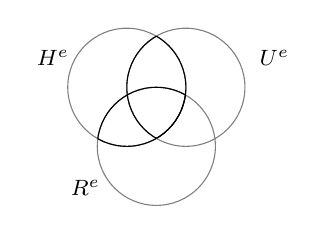
\begin{tikzpicture}[scale=.75]
\def\circleH{(0,1) circle (1cm)}
\def\circleU{(1,1) circle (1cm)}
\def\circleR{(.5,0) circle (1cm)}
\draw[gray] \circleH;
\draw[gray] \circleU;
\draw[gray] \circleR;
\begin{scope}
  \clip \circleH;
  \draw \circleU;
  \draw \circleR;
\end{scope}
\begin{scope}
  \clip \circleU;
  \draw \circleH;
\end{scope}
\begin{scope}
  \clip \circleR;
  \draw \circleH;
\end{scope}
\node at (-1.25,1.5) {\footnotesize{$H^e$}};
\node at (2.5,1.5) {\footnotesize{$U^e$}};
\node at (-.7,-.7) {\footnotesize{$R^e$}};
%\node at (.5,2.25) {\footnotesize{$u^e$}};
%\node at (.5,1.4) {\footnotesize{$\bar{r}_{e}$}};
%\node at (.5,.55) {\footnotesize{$r^e$}};
\end{tikzpicture}
&
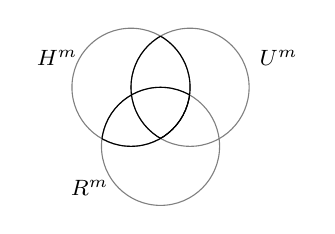
\begin{tikzpicture}[scale=.75]
\def\circleH{(0,1) circle (1cm)}
\def\circleU{(1,1) circle (1cm)}
\def\circleR{(.5,0) circle (1cm)}
\draw[gray] \circleH;
\draw[gray] \circleU;
\draw[gray] \circleR;
\begin{scope}
  \clip \circleH;
  \draw \circleU;
  \draw \circleR;
\end{scope}
\begin{scope}
  \clip \circleU;
  \draw \circleH;
\end{scope}
\begin{scope}
  \clip \circleR;
  \draw \circleH;
\end{scope}
\node at (-1.25,1.5) {\footnotesize{$H^m$}};
\node at (2.5,1.5) {\footnotesize{$U^m$}};
\node at (-.7,-.7) {\footnotesize{$R^m$}};
%\node at (.5,2.25) {\footnotesize{$u^e$}};
%\node at (.5,1.4) {\footnotesize{$\bar{r}_{e}$}};
%\node at (.5,.55) {\footnotesize{$r^e$}};
\end{tikzpicture}
\\
\mc{2}{c}{Model and regression design:}\\
\mc{2}{l}{11: $(U^e \cap H^e) \rightarrow (R^e \cap H^e)$}\\
\mc{2}{l}{12: $(U^e \cap H^e) \rightarrow (R^m \cap H^m)$}\\
\mc{2}{l}{13: $(U^m \cap H^m) \rightarrow (R^e \cap H^e)$}\\
\mc{2}{l}{14: $(U^m \cap H^m) \rightarrow (R^m \cap H^m)$}\\
\mc{2}{l}{15: $U^e \rightarrow R^e$}\\
\mc{2}{l}{16: $U^e \rightarrow R^m$}\\
\end{tabular}
\caption{Proposal subsets analyzed in lagged weekly urgency models}\label{f:vennNegBin}
\end{figure}

Other controls in the right side, all measured at week $t$, are net presidential aproval, the percentage of the term remaining (executive and C\'amara were elected concurrently in the period), and a dummy distinguishing the 2010--2014 Legislature from the 2006--2010 baseline. Weeks when the chamber did not meet were dropped, adding any of that week's reports to the closest next week with a session. Bill histories date reports when officially received by chamber staff (when they entered the so-called \emph{cuenta}, the official tally), which may be days before plenary announcement. The algorithm coded these dates incorrectly, explaining reports dated in session-less weeks. The same could happen for weekly urgency messages, corrected likewise.

The median C\'amara session week in the period had one bill reported by Hacienda and four by any committee (with deviations of 1.5 and 5.9, respectively). Given the limited nature of the dependent variable (a count), negative binomial regression was used for estimation \citep{cameron.trivedi.1998}. 

Table \ref{t:appendixNreportNegBin} reports regression fit (need to replicate rest of regressions, or drop them from text!)

% Table created by stargazer v.5.2 by Marek Hlavac, Harvard University. E-mail: hlavac at fas.harvard.edu
% Date and time: Mon, Nov 09, 2015 - 08:20:10 PM
% Requires LaTeX packages: dcolumn 
\begin{table} \centering 
\begin{tabular}{@{\extracolsep{5pt}}lD{.}{.}{-3} D{.}{.}{-3} } 
 & \multicolumn{1}{c}{(11)} & \multicolumn{1}{c}{(15)}\\ 
\hline \\[-1.8ex] 
 \emph{nActNow} & 0.370^{***} & 0.262^{***} \\ 
  & p = 0.000 & p = 0.000 \\ [.75ex]
 \emph{nActNowLag1} & 0.189^{**} & 0.099^{**} \\ [.75ex]
  & p = 0.012 & p = 0.043 \\ 
 \emph{nActNowLag2} & -0.217^{**} & -0.259^{***} \\ 
  & p = 0.029 & p = 0.00001 \\ [.75ex]
 \emph{n2weekLag1} & 0.099^{***} & 0.035^{**} \\ 
  & p = 0.0002 & p = 0.019 \\ [.75ex]
 \emph{n2weekLag2} & 0.002 & 0.019 \\ 
  & p = 0.946 & p = 0.256 \\ [.75ex]
 \emph{n2weekLag3} & -0.056 & 0.023 \\ 
  & p = 0.166 & p = 0.168 \\ [.75ex]
 \emph{n1monthLag2} & -0.026 & 0.001 \\ 
  & p = 0.520 & p = 0.933 \\ [.75ex]
 \emph{n1monthLag3} & 0.088^{**} & 0.013 \\ 
  & p = 0.012 & p = 0.421 \\ [.75ex]
 \emph{n1monthLag4} & 0.060^{**} & 0.015 \\ 
  & p = 0.049 & p = 0.279 \\ [.75ex]
 \emph{nShorten} & 0.086 & 0.065 \\ 
  & p = 0.202 & p = 0.182 \\ [.75ex]
 \emph{nShortenLag1} & 0.177^{**} & 0.089^{*} \\ 
  & p = 0.017 & p = 0.091 \\ [.75ex]
 \emph{nShortenLag2} & -0.016 & -0.057 \\ 
  & p = 0.864 & p = 0.330 \\ [.75ex]
 \emph{Term remaining} & 0.001 & -0.001 \\ 
  & p = 0.528 & p = 0.636 \\ [.75ex]
 \emph{Pres.~approval} & -0.006^{**} & -0.006^{***} \\ 
  & p = 0.023 & p = 0.0002 \\ [.75ex]
 \emph{2010--14 Leg.} & -0.479^{***} & -0.354^{***} \\ 
  & p = 0.002 & p = 0.0003 \\ [.75ex]
 Constant & 0.024 & 1.200^{***} \\ 
  & p = 0.904 & p = 0.000 \\ [.75ex]
\hline \\[-1.8ex] 
Observations & \multicolumn{1}{c}{309} & \multicolumn{1}{c}{309} \\ 
Log Likelihood & \multicolumn{1}{c}{$-419.3$} & \multicolumn{1}{c}{$-635.6$} \\ 
%$\theta$ & \multicolumn{1}{c}{11,192.890  (123,036.000)} & \multicolumn{1}{c}{19.122^{*}  (10.630)} \\ 
%Akaike Inf. Crit. & \multicolumn{1}{c}{870.560} & \multicolumn{1}{c}{1,303.257} \\ 
\hline \\[-1.8ex] 
  & \multicolumn{2}{r}{\footnotesize{$^{*}$p$<$.1; $^{**}$p$<$.05; $^{***}$p$<$.01 (two-tailed tests)}} \\ 
\end{tabular} 
  \caption{Negative binomial regressions of \emph{nReports}$_t$} 
  \label{t:appendixNreportNegBin} 
\end{table} 


% recover regression tables and report in the appendix; estimate senate versions and report

%It includes the C\'amara's spontaneous reports and reports presumably triggered by urgency message. If the urgency authority is consequential, the number and type of weekly urgency messages should correlate with total weekly reports. 

%Two quantities were aggregated for analysis: weekly Hacienda committee reports, and weekly reports from any committee. The Hacienda aggregate seems preferable, letting analysis search for correlation with urgency messages explicitly targeting bills that were referred to that committee. The total aggregate offers less control, but a more comprehensive picture. 

%Analysis, at this stage, does not control for exceptions to the post-urgency report expectation, such as bills that had been reported before the urgency message was issued. But, unless there is a reason to suspect that most or many urgency messages arrive after the committee has reported---and I see no a priori reason to expect this---a relatively large number of messages should be followed by a report. And the report's timing should bear relation to the degree of the urgency. 

% Maybe useful to close the appendix subsection
%Inspection of Hacienda committee scheduling and activity in detail should prove illuminating. Qualitative inspection of the issues declared urgent, of the urgency messages and their content (especially the recommendations that the messages communicate), and of committee reports themselves will shed light on whether or not, and how cost $k$ is supporting a consequential urgency authority in Chile. The level of urgency results certainly do. 

%% APPENDIX SUBSECTION ENDS HERE



\bibliographystyle{apsr}
\bibliography{/home/eric/Dropbox/mydocs/magar}

\end{document}

